%%%%%%%%%%%%%%%%%%%%%%%%%%%%%%%%%%%%%%%%%
% Masters/Doctoral Thesis 
% LaTeX Template
% Version 2.5 (27/8/17)
%
% This template was downloaded from:
% http://www.LaTeXTemplates.com
%
% Version 2.x major modifications by:
% Vel (vel@latextemplates.com)
%
% This template is based on a template by:
% Steve Gunn (http://users.ecs.soton.ac.uk/srg/softwaretools/document/templates/)
% Sunil Patel (http://www.sunilpatel.co.uk/thesis-template/)
%
% Template license:
% CC BY-NC-SA 3.0 (http://creativecommons.org/licenses/by-nc-sa/3.0/)
%
%%%%%%%%%%%%%%%%%%%%%%%%%%%%%%%%%%%%%%%%%

%----------------------------------------------------------------------------------------
%	PACKAGES AND OTHER DOCUMENT CONFIGURATIONS
%----------------------------------------------------------------------------------------

\documentclass[
11pt, % The default document font size, options: 10pt, 11pt, 12pt
%oneside, % Two side (alternating margins) for binding by default, uncomment to switch to one side
serbian, % ngerman for German
singlespacing, % Single line spacing, alternatives: onehalfspacing or doublespacing
%draft, % Uncomment to enable draft mode (no pictures, no links, overfull hboxes indicated)
%nolistspacing, % If the document is onehalfspacing or doublespacing, uncomment this to set spacing in lists to single
%liststotoc, % Uncomment to add the list of figures/tables/etc to the table of contents
%toctotoc, % Uncomment to add the main table of contents to the table of contents
%parskip, % Uncomment to add space between paragraphs
% nohyperref, % Uncomment to not load the hyperref package
headsepline, % Uncomment to get a line under the header
%chapterinoneline, % Uncomment to place the chapter title next to the number on one line
%consistentlayout, % Uncomment to change the layout of the declaration, abstract and acknowledgements pages to match the default layout
]{MastersDoctoralThesis} % The class file specifying the document structure

\usepackage[utf8]{inputenc} % Required for inputting international characters
\usepackage[T1]{fontenc} % Output font encoding for international characters

\usepackage{mathpazo} % Use the Palatino font by default
\usepackage{amsmath}
% dužine

\usepackage[backend=bibtex,style=authoryear,natbib=true]{biblatex} % Use the bibtex backend with the authoryear citation style (which resembles APA)

\addbibresource{ref.bib} % The filename of the bibliography

\usepackage[autostyle=true]{csquotes} % Required to generate language-dependent quotes in the bibliography

%----------------------------------------------------------------------------------------
%	MARGIN SETTINGS
%----------------------------------------------------------------------------------------

\geometry{
	paper=a4paper, % Change to letterpaper for US letter
	inner=2.5cm, % Inner margin
	outer=3.8cm, % Outer margin
	bindingoffset=.5cm, % Binding offset
	top=1.5cm, % Top margin
	bottom=1.5cm, % Bottom margin
	%showframe, % Uncomment to show how the type block is set on the page
}

%----------------------------------------------------------------------------------------
%	THESIS INFORMATION
%----------------------------------------------------------------------------------------

\thesistitle{Računarska analiza povezanosti funkcije i neuređenosti proteina} % Your thesis title, this is used in the title and abstract, print it elsewhere with \ttitle
\supervisor{dr. Jovana \textsc{Kovačević}} % Your supervisor's name, this is used in the title page, print it elsewhere with \supname
\examiner{} % Your examiner's name, this is not currently used anywhere in the template, print it elsewhere with \examname
\degree{Master informatičar} % Your degree name, this is used in the title page and abstract, print it elsewhere with \degreename
\author{Goran \textsc{Vinterhalter}} % Your name, this is used in the title page and abstract, print it elsewhere with \authorname
\addresses{https://www.linkedin.com/in/goran-vinterhalter-6996a412b/} % Your address, this is not currently used anywhere in the template, print it elsewhere with \addressname

\subject{Bioinformatika} % Your subject area, this is not currently used anywhere in the template, print it elsewhere with \subjectname
\keywords{} % Keywords for your thesis, this is not currently used anywhere in the template, print it elsewhere with \keywordnames
\university{\href{http://www.bg.ac.rs}{Univerzitet u Beogradu}} % Your university's name and URL, this is used in the title page and abstract, print it elsewhere with \univname
\department{\href{http://www.racunarstvo.matf.bg.ac.rs/}{Katedra za Računarstvo i informatiku}} % Your department's name and URL, this is used in the title page and abstract, print it elsewhere with \deptname
\group{.} % Your research group's name and URL, this is used in the title page, print it elsewhere with \groupname
% \group{\href{http://researchgroup.university.com}{Research Group Name}} % Your research group's name and URL, this is used in the title page, print it elsewhere with \groupname
\faculty{\href{http://matf.bg.ac.rs}{Matematički fakultet}} % Your faculty's name and URL, this is used in the title page and abstract, print it elsewhere with \facname

\AtBeginDocument{
\hypersetup{pdftitle=\ttitle} % Set the PDF's title to your title
\hypersetup{pdfauthor=\authorname} % Set the PDF's author to your name
\hypersetup{pdfkeywords=\keywordnames} % Set the PDF's keywords to your keywords
}

\begin{document}

\frontmatter % Use roman page numbering style (i, ii, iii, iv...) for the pre-content pages

\pagestyle{plain} % Default to the plain heading style until the thesis style is called for the body content

%----------------------------------------------------------------------------------------
%	TITLE PAGE
%----------------------------------------------------------------------------------------

\begin{titlepage}
\begin{center}

\vspace*{.06\textheight}
{\scshape\LARGE \univname\par} % University name
{\scshape\LARGE \facname\par} % University name
\vspace{1.5cm}
\textsc{\Large Master Rad}\\[0.5cm] % Thesis type

\HRule \\[0.4cm] % Horizontal line
{\huge \bfseries \ttitle\par}\vspace{0.4cm} % Thesis title
\HRule \\[1.5cm] % Horizontal line
 
\begin{minipage}[t]{0.4\textwidth}
\begin{flushleft} \large
\emph{Autor:}\\
\href{https://www.linkedin.com/in/goran-vinterhalter-6996a412b/}{\authorname} % Author name - remove the \href bracket to remove the link
\end{flushleft}
\end{minipage}
\begin{minipage}[t]{0.4\textwidth}
\begin{flushright} \large
\emph{Mentor:} \\
\href{http://poincare.matf.bg.ac.rs/~jovana/}{\supname} % Supervisor name - remove the \href bracket to remove the link  
\end{flushright}
\end{minipage}\\[2cm]
 
\vfill

% \large \textit{A thesis submitted in fulfillment of the requirements\\ for the degree of \degreename}\\[0.3cm] % University requirement text
% \textit{in the}\\[0.4cm]
% \groupname\\\deptname\\[2cm] % Research group name and department name

{\scshape\LARGE Članovi komsije:\par}\vspace{0.2cm} % University name
prof. dr Gordana Pavlović-Lažetić \\
prof. dr Saša Malkov \\
prof. dr Jovana Kovačević \\

 
\vfill

\vspace{1cm}
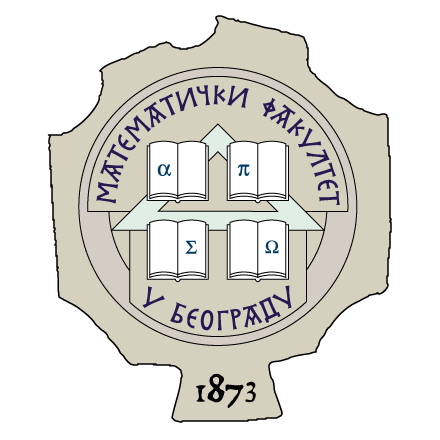
\includegraphics[scale=0.25]{Logo}\\ % University/department logo - uncomment to place it
\vspace{0.5cm}
{\large Beograd, 2017}\\ % Date
 
\vfill
\end{center}
\end{titlepage}

%----------------------------------------------------------------------------------------
%	DECLARATION PAGE
%----------------------------------------------------------------------------------------

% \begin{declaration}
% \addchaptertocentry{\authorshipname} % Add the declaration to the table of contents
% \noindent I, \authorname, declare that this thesis titled, \enquote{\ttitle} and the work presented in it are my own. I confirm that:
%
% \begin{itemize} 
% \item This work was done wholly or mainly while in candidature for a research degree at this University.
% \item Where any part of this thesis has previously been submitted for a degree or any other qualification at this University or any other institution, this has been clearly stated.
% \item Where I have consulted the published work of others, this is always clearly attributed.
% \item Where I have quoted from the work of others, the source is always given. With the exception of such quotations, this thesis is entirely my own work.
% \item I have acknowledged all main sources of help.
% \item Where the thesis is based on work done by myself jointly with others, I have made clear exactly what was done by others and what I have contributed myself.\\
% \end{itemize}
%  
% \noindent Signed:\\
% \rule[0.5em]{25em}{0.5pt} % This prints a line for the signature
%  
% \noindent Date:\\
% \rule[0.5em]{25em}{0.5pt} % This prints a line to write the date
% \end{declaration}
%
% \cleardoublepage

%----------------------------------------------------------------------------------------
%	QUOTATION PAGE
%----------------------------------------------------------------------------------------

% \vspace*{0.2\textheight}
%
% \noindent\enquote{\itshape Thanks to my solid academic training, today I can write hundreds of words on virtually any topic without possessing a shred of information, which is how I got a good job in journalism.}\bigbreak
%
% \hfill Dave Barry

%----------------------------------------------------------------------------------------
%	ABSTRACT PAGE
%----------------------------------------------------------------------------------------

\begin{abstract}
\addchaptertocentry{\abstractname} % Add the abstract to the table of contents
The Thesis Abstract is written here (and usually kept to just this page). The page is kept centered vertically so can expand into the blank space above the title too\ldots
\end{abstract}

%----------------------------------------------------------------------------------------
%	ACKNOWLEDGEMENTS
%----------------------------------------------------------------------------------------

% \begin{acknowledgements}
% \addchaptertocentry{\acknowledgementname} % Add the acknowledgements to the table of contents
% The acknowledgments and the people to thank go here, don't forget to include your project advisor\ldots
% \end{acknowledgements}
%
%----------------------------------------------------------------------------------------
%	LIST OF CONTENTS/FIGURES/TABLES PAGES
%----------------------------------------------------------------------------------------

\tableofcontents % Prints the main table of contents

% \listoffigures % Prints the list of figures

% \listoftables % Prints the list of tables

%----------------------------------------------------------------------------------------
%	ABBREVIATIONS
%----------------------------------------------------------------------------------------

\begin{abbreviations}{ll} % Include a list of abbreviations (a table of two columns)

\textbf{LAH} & \textbf{L}ist \textbf{A}bbreviations \textbf{H}ere\\
\textbf{WSF} & \textbf{W}hat (it) \textbf{S}tands \textbf{F}or\\

\end{abbreviations}

%----------------------------------------------------------------------------------------
%	PHYSICAL CONSTANTS/OTHER DEFINITIONS
%----------------------------------------------------------------------------------------

% \begin{constants}{lr@{${}={}$}l} % The list of physical constants is a three column table
%
% % The \SI{}{} command is provided by the siunitx package, see its documentation for instructions on how to use it
%
% Speed of Light & $c_{0}$ & \SI{2.99792458e8}{\meter\per\second} (exact)\\
% %Constant Name & $Symbol$ & $Constant Value$ with units\\
%
% \end{constants}

%----------------------------------------------------------------------------------------
%	SYMBOLS
%----------------------------------------------------------------------------------------

% \begin{symbols}{lll} % Include a list of Symbols (a three column table)
%
% $a$ & distance & \si{\meter} \\
% $P$ & power & \si{\watt} (\si{\joule\per\second}) \\
% %Symbol & Name & Unit \\
%
% \addlinespace % Gap to separate the Roman symbols from the Greek
%
% $\omega$ & angular frequency & \si{\radian} \\
%
% \end{symbols}

%----------------------------------------------------------------------------------------
%	DEDICATION
%----------------------------------------------------------------------------------------

% \dedicatory{For/Dedicated to/To my\ldots} 

%----------------------------------------------------------------------------------------
%	THESIS CONTENT - CHAPTERS
%----------------------------------------------------------------------------------------

\mainmatter % Begin numeric (1,2,3...) page numbering

\pagestyle{thesis} % Return the page headers back to the "thesis" style

% definišemo korisne komande
\newcommand{\en}[1]{(engl. \textit{#1})}
\newcommand{\keyword}[1]{ \textbf{#1}  }
\newcommand{\tabhead}[1]{ \textbf{#1}  }
\newcommand{\code}[1]{ \texttt{#1}  }
\newcommand{\file}[1]{ \texttt{\bfseries#1}  }
\newcommand{\option}[1]{ \texttt{\itshape#1}  }

% Include the chapters of the thesis as separate files from the Chapters folder
% Uncomment the lines as you write the chapters


\chapter{Uvod} % Main chapter title

\label{Uvod} % For referencing 


%------------------------------------------------------------------------------

\section{Osnovni biološki  pojmovi}

Svi živi organizmi sastoje se od jedne ili više ćelija, a svaka ćelija od
molekula. Veliki \footnote{ Obično se molekulska masa od $1000 Da$ (Daltona) uzima kao 
granica između malih molekula i makromolekula.}
molekuli (makromolekuli) organskog porekla obično \footnote{
  Lipidi recimo nisu polimeri, ali su principijalno slični
} su sačinjeni od
ponavljajućih strukturnih jedinica \keyword{monomera} \textit{(mono- = jedan,
mer- = deo)} međusobno povezanih \keyword{kovalentnim} vezama.  Takav molekul
zovemo \keyword{polimer} \textit{(poli- =mnogo, -mer= deo)}. 
% Polimer može da bude \textit{homo-polimer}, sačinjen od jednog tipa monomera
% ili suprotno \textit{hetero-polimer}, sačinjen od nekoliko raznih tipova
% monomera.
Skup monomera možemo da smatramo azbukom koja gradi jezik polimera.  Mali broj
monomera je dovoljan za strukturnu kompleksnost bilo koje ćelije.  Tri 
najznačajnija tipa bioloških polimera i njihovi monomeri prikazani su u Tabli
\ref{tab:polimeri}.

\begin{table}[htpb]
  \centering
  \caption{Najznačajniji biološki polimeri}
  \label{tab:polimeri}
  \begin{tabular}{ll}
    \keyword{Polimer}            & \keyword{Monomer} \\
    Ugljeni hidrati              & Monosaharid (šećeri) \\
    Nukleinska kiselina (DNK)    & Nukleotid \\
    Protein                      & Aminokiselina \\
    \hline
  \end{tabular}
\end{table}



\label{sec:}
\subsection{Proteini}

Proteini su najčešći biološki makromolekuli koji čine i do $80\%$ suve mase
organizma.  Strukturno protein je linearan polimeri sačinjen od lanca
\keyword{aminokiselina}(monomeri). 





\chapter{Podaci i metode} % Main chapter title

\label{Podaci i metode} % For referencing 

Cilj rada je ispitivanje veze između molekulske funkcije proteina i njegove
(ne)ure- đenosti tj. da li molekulska funkcija zavisi više od uređenosti ili
neuređenosti. Istraživanje je motivisano radom\parencite{Xie2007}. Navedeni rad
je prvi u seriji od tri rada i bavi se prvenstveno biološkim procesima i
molekulskim funkcijama.  U nastavku teksta pod terminima \keyword{originalni}
rad, autori, podaci, metode i slično podrazumevaćemo navedeni rad, njegove
autore, metode, podatke itd.

Najveća razlika u pristupu između originalnog i ovog istraživanja je što su
originalni rezultati izraženi u terminima \keyword{ključnih reči} dok su ovde
rezultati izraženi u \keyword{GO terminima}. Oba pristupa proizvode listu
funkcija koje više obuhvataju (ne)uređene proteine, ali GO termini zbog
granularnosti se prirodnije predstavljaju grafovski i sadrže mnogo više
funkcija. Jedan od rezultata ovog istraživanja predstavlja poređenje ova dva
pristupa.


\section {Podaci}

Za metode koje prezentujemo potrebne su tri vrste informacija:
\begin{enumerate}
  \item Što više različitih proteina
  \item Pouzdana anotacija funkcija
  \item Informacije o funkcijama, prvenstveno međurelacije (međurelacije između\\ funkcija su bitne  ako ih je potrebno grupisati)
\end{enumerate}


\subsection{Podaci iz originalnog rada}

U originalnom radu \parencite{Xie2007} korišćena je  baza podataka 
\keyword{\swissprot} (Poglavlje \ref{svis-prot}), verzija 48 iz 2005.
Verzija 48 ima 201 560 proteina od kojih 196 326 imaju dužinu preko 40
aminokiselina (što je potrebno zbog Definicije \ref{pdis_def} u nastavku). Funkcije
pridružene proteinima izražene su \keyword{kontrolisanim vokabularom}
\en{controlled vocabulary} koga čine takozvane \textit{UniProtKB} \keyword{ključne reči}
\en{keywords}. U verziji 48, UniProtKB sadrži 874 ključnih reči.  Zbog
statističke značajnosti posmatrane su one ključne reči kojima je bilo anotirano
barem 20 proteina, tj. 710 ključnih reči.

Kao što je pomenuto u Poglavlju \ref{svis-prot}, kanonske sekvence (proteini) u \swissprot
bazi podataka nisu redundantne u smislu da jedan unos u bazi podataka predstavlja produkt
jednog gena iz jedne vrste organizma. Međutim, za analizu funkcija
\swissprot \keyword{jeste statistički redundantna} \parencite{Xie2007} jer
sadrže veliku količinu \keyword{homologih} proteina (prvenstveno ortologa).
Zbog statističke redundantnosti originalni autori su izvršili klasterovanje \swissprot
proteina u \keyword{proteinske familije} dobivši 27 217 familija. Posledica
klasterovanja je da svaki protein dobija težinu kojom doprinosi daljoj analizi.
Težina svakog proteina u preseku klastera sa datom funkcijom je obrnuto
proporcionalna veličini preseka tako da je zbir težina svih proteina jednaka
veličini preseka.

% \textbf{komentar:} \\
% Ono što autori nisu elaborirali jeste da početni uslov od minimum 20 proteina
% po ključnoj reči možda nije dovoljan. Ako pretpostavimo zarad ilustracije
% normalnu raspodelu veličina klastera proteina, očekivali bi da klaster najčešće
% sadrži 7 proteina. Dakle iako je 50 proteina pridruženo nekoj funkciji ona
% verovatno ima pridruženih svega 7 familija proteina. Kako familija sadrži
% proteine pod pretpostavkom istog evolutivnog porekla njihova funkcija bi
% trebalo da je slična pa se onda postavlja pitanje da li je 7 familija dovoljno
% da bi se razmatrala data ključna reč. Ovo je primarno kritika za ključne reči
% jer one obično predstavljaju opšte pojmove.
%
% Sa druge strane za usko specijalizovane pojmove bila bi dovoljna jedna familija
% proteina jer bi ona predstavljala sve razne homologe (TODO Burkhard Rost,
% Termofili)

\subsection{Podaci korišćeni u ovom istraživanju}

Ugledom na \keyword{CASP} takmičenja, \keyword{CAFA} \en{Critical Assessment of
Functional Annotation} takmičenje pokrenuto je zarad objektivnog ocenjivanja
prediktora funkcije proteina i usmeravanja budućeg razvoja ove oblasti
\parencite{CAFA}.  U ovom radu korišćen je trening skup proteina preuzet sa
\keyword{CAFA3} takmičenja, održanog 2017. Trening skupovi su podaci na osnovu
kojih prediktor uči, pa shodno tome ovaj skup treba da predstavlja dobar uzorak
proteina odnosno njihovih funkcija.

CAFA3 trening skup (u nastavku samo CAFA3 skup ili CAFA3 podaci) je podskup \swissprot baze (iz 2016.) koji
uključuje proteine iz model organizama: \textit{Human, Mouse, Rat, S.
cerevisiae, S. pombe, E. coli, A. thaliana, Dictyostelium discoideum,
Zebrafish, Bacillus cereus} sa izuzetokm sekvenci \textit{Drosophila} i \textit{Candida}
koje su preuzete iz svojih genomskih baza podataka, respektivno.
Slika \ref{fig:sp_vs_cafa3} pruža detaljan taksonomski uvid o poreklu CAFA3 proteina.
Na primer, \swissprot baza sadrži oko 20 000 ljudskih (\textit{Homo})
proteinskih sekvenci dok CAFA3 podskup sadrži malo manje od 15 000.  Vrste
koje doprinose sa manje od 100 proteina nisu prikazane radi kompaktnosti.

\begin{figure}[th]
\centering
\hspace*{-3.0cm} 
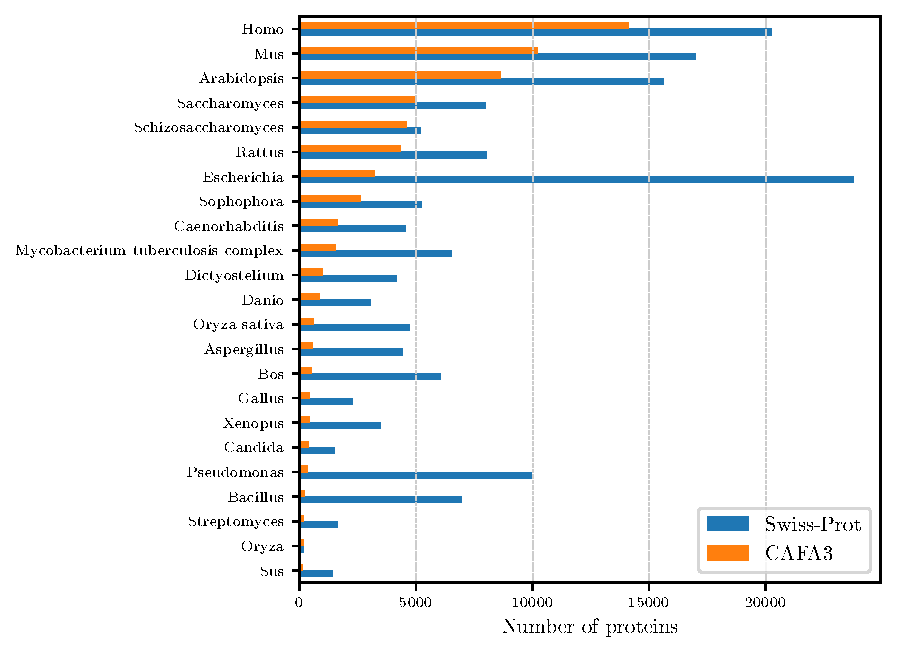
\includegraphics[]{plots/sp_vs_cafa3}
% \decoRule
\caption{Taksonomsko poreklo CAFA3 proteina. \\ \footnotesize 
}
\label{fig:sp_vs_cafa3}
\end{figure}

Za razliku od proteina u \swissprot bazi čije je postojanje pretežno utvrđeno
iz homologije, $74\%$ proteina iz CAFA3 podskupa identifikovani su na nivou
nivou proteina što je najveći stupanj sigurnosti da proteini zaista postoji. Na
Slici \ref{fig:cafa3_pe} ilustrovana je razlika u odnosu na pouzdanost
postojanja proteina. 



\begin{figure}[th]
\centering
\hspace*{-2.5cm} 
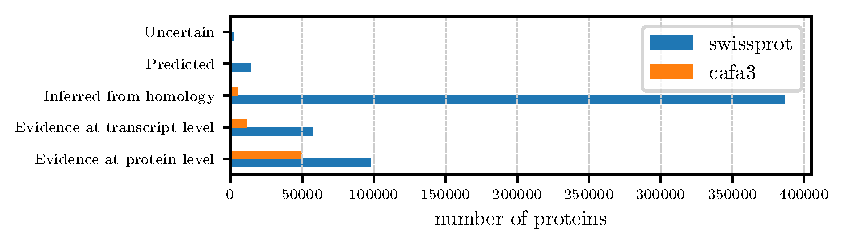
\includegraphics[]{plots/cafa3_pe}
% \decoRule
\caption{Razlika izmedju pouzdanosti postojanja proteina iz \\ \swissprot baze i njenog CAFA3 podskupa. }
\label{fig:cafa3_pe}
\end{figure}


Važno je naglasiti da je dalja analiza izvršena pod pretpostavkom da CAFA3 skup
nije statistički redundantan, što znači da klasterovanje u proteinske familije
nije potrebno.  Isključivanje ove pretpostavke bi dovelo do komplikovanijih
računarskih metoda za analizu što je van opsega ovog rada.



% Iako ovaj pristup potencijalno proizvodi skup koji je \keyword{statisički
% redundantan} u našoj analizi smo pretpostavili da to nije slučaj jer je čin
% klasterovanja veoma računarski zahtevan, a nismo ubeđeni da je neophodan za
% ovaj konkretan skup. Iz tog razloga u daljoj analizi predstavljamo uprošćenu
% verziju formule koja ne uračunva težinu pojedinačnog proteina.

\swissprot proteini su kodirani jednim karakterom koristeći \keyword{IUPAC}
kodove.  U podacima javljaju se sekvence sa  21. i 22. aminokiselinom ('U' i 'O')
kao i  višeznačne oznake: 'B', 'J', 'X' i 'Z'.  Ovakve sekvence nisu podržane od
strane VSL2b prediktora i za nas predstavljaju nevalidne proteinske sekvence. Pod
\keyword{validnom proteinskom sekvencom} smatraćemo sekvencu koja je validan
ulaz za VSL2b, tj. čini je azbuka od 20 standardnih aminokiselina i
ima minimalnu dužinu 9 AK.

CAFA3 Podaci se sastoje od dve datoteke:
\begin{enumerate}
  \item \file{uniprot\_sprot\_exp.fasta}  sadrži 66 841 protein od kojih 66 599
    za našu analizu predstavljaju validnu proteinsku sekvencu. Od preostalih
    proteina 66 063 ima dužinu veću ili jednaku od 40 aminokiselina.
  \item \file{uniprot\_sprot\_exp.txt} proteinima pridružuje funkcije u obliku 
    \keyword{GO termina}. Zastupljeni su termini iz sva tri imenska prostora:
    16 117 ćelijskih komponenti, 5 966 molekulskih funkcija i 16 117 bioloških
    procesa. Jednom proteinu može biti pridruženo više GO termina i obrnuto.
\end{enumerate}

Analiza u ovom radu je primarno orijentisna ka korišćenju GO termina za opis
funkcije što je razlikuje od originalnog pristupa korišćenja ključnih reči.
Analiza GO termina zahteva poznavanje prvenstveno \textit{is\_a} roditeljske
veze između termina. Takođe, tokom istraživanja bile su nam potrebne i ostale
informacije o terminima. Pomenute informacije dobili smo iz datoteke
\file{go.obo} \cite{go_obo} verzije 01.12.2017.

Odnos tj. mapiranje između ključnih reči i GO termina dostupno je sa dva izvora:
\begin{itemize}
  \item \file{keywlist.txt}\cite{keywlist_txt} verzija 20.12.2017 sadrži
    informacije o 1188 ključnih reči od kojih 195 pripada kategoriji
    \keyword{Molekulskih funkcija}. Više o mapiranju biće
    izloženo u Potpoglavlju \ref{kw2go_mapiranje}.
  \item \file{uniprotkb\_kw2go}\cite{uniprotkb_kw2go} sadrži samo mapiranja a
    generiše ih \keyword{GOA projekat} \parencite{Barrell2009}. 
\end{itemize}

U ovom radu korišćena je isključivo \file{keywlist.txt} datoteka. Iako je
datoteka \\ \file{uniprot\_kw2go} sadržala veći broj mapiranja, unosila je
nepoželjnu višeznačnost.

Pošto je originalni rad iz 2007. godine, postoje razlike u broju proteina,
anotacijama ključnih reči, broju ključnih reči ali i primarnoj strukturi proteinskih
sekvenci.  Radi procene uticaja navedenih razlika na rezultat, odlučeno je da se
analiza prvo ponovi originalnim pristupom, koristeći vokabular ključnih reči.
Iz tog razloga, CAFA3 podaci nisu mogli da se posmatraju kao crne kutije, već
je bilo neophodno mapirati ih nazad na \swissprot proteine čije su anotacije 
ključnim rečima poznate. Ovaj korak objedinjavanja baza podataka opisan je u
Potpoglavlju \ref{objedinjavanje}. Dobijene anotacije ključnim rečima takođe su
iskorišćene za proveru validnosti mapiranja ključnih reči na GO termine.
Mapiranja su detaljno opisana u Potpoglavlju \ref{kw2go_mapiranje}



\section {Metod}


Pod \keyword{idealnim slučajem},
pretpostavimo da za proizvoljnu molekulsku funkciju znamo sve strukturno različite
proteine koji je obavljaju.  Da bi dali korektan odgovor  moramo da znamo kako
neuređenost pojedinačnog proteina utiče na
na njegovo ponašanje, i kako to ponašanje (tip neuređenosti) utiče na datu funkciju.
% Ova vrsta znanja nije bila dostupna 2007. osim za jako mali skup proteina.

Nažalost, ograničenja današnjih podataka i razvijenih metoda su brojna:
\begin{itemize}
  \item
    Baza eksperimentalno utvrđenih neuređenih regiona
    \textit{\keyword{DisProt}} ima svega 803 proteina sa opisanih 2167
    neuređenih regiona \parencite{Piovesan2016}.  Uz to, kvalitet navedenih
    informacija je diskutabilan zbog razlika u pouzdanosti među
    eksperimentalnim tehnikama koje su korišćene.  Najveću pouzdanost nose
    regioni koji su eksperimentalno okarakterisani sa što većim brojem
    laboratorijskih tehnika.

  \item
    Prediktori se treniraju na malom podskupu proteina iz \textit{DisProt}
    i PDB  baze. Čak i konsenzus nekoliko različitih prediktora ne daje
    dovoljno pouzdane rezultate o lokaciji neuređenog regiona.

  \item 
    Pozitivna strana je najnoviji napredak, razvoj prediktora koji direktno
    pokušavaju da predvide funkciju koju IDPr obavlja \parencite{Meng_c2017}.
  % \item Koliko nam je poznato trenutno nema prediktora koji predviđaju tip
  %   neuređenosti. Takođe, Opisivanje tipa neuređenosti predstavlja poduhvat.
  %   \begin{itemize}
  %     \item Prof. Vladimir Uverski predlaže nekoliko imena za opis različitih
  %       ponašanja neuređenih proteina \en{Folldon, Unfolldon, ...}
  %       \parencite{Uversky2017}.
  %     \item Prof. Peter Tompa je zaslužan za kreiranje 3 ontologije neuređenih
  %       regiona za bazu Disprot koji precizno modeluje tipove
  %       neuređenosti \parencite{disprot}.  .  Međutim koliko nam je poznato
  %       prediktori koji predviđaju termine ove ontologije još nisu napravljeni
  %   \end{itemize}

\end{itemize}

Jednostavna alternativa idealnom slučaju je da se pretpostavi da veći udeo neuređenih u odnosu
na uređene proteine podrazumeva da funkcija zavisi više od neuređenosti. 
% Dakle izjednačavamo uzročnost \en{causation} i \keyword{korelaciju} između funkcije i neuređenosti.
% Međutim, prvo je potrebno precizirati kada protein smatramo neuređenim.
% Definicija mora da ima biološkog smisla, da bude prilagođena
% analizi, ali pored takođe je ograničena sposobnostima i preciznošću prediktora
% koji se korist.  Više o tome u narednom Potpoglavlju \ref{naredno}.

\subsection{Predikcija neuređenosti proteina}
\label{naredno}

Originalni autori koristili su \keyword{PONDR VL3E} prediktor koji
postiže tačnost od $~87\%$ pri unakrsnoj validaciji nad uravnoteženim test
skupom.  Zbog ekonomičnosti i dostupnosti u ovom radu korišćen je noviji
prediktor druge generacije \keyword{PONDR VSL2b}.
Relevantne karakteristike VSL2b prediktora detaljno su opisane u \ref{VSL2b}.
Za potrebe analize originalni autori  uvode sledeću definiciju:

\newtheorem{mydef}{Definicija}
\begin{mydef}
\label{pdis_def}
Protein je \keyword{putativno neuređen} (najverovatnije neuređen, u daljem tekstu neuređen) engl. putatively disordered
ako sadrži bar jedan region veći ili jednak od 40 uzastopnih aminokiselina
takvih da im je predviđenu neuređenost iznad 0.5. 
\end{mydef}

Onda definišemo operator $d$ takav da za svaku proteinsku sekvencu $s_i$ važi:

\[   
  d(s_i) = 
    \begin{cases}
      1 & \text{ako je} \quad s_i \quad \keyword{neuređena}\\
      0 & \text{suprotno}
    \end{cases}
\]

Uslov ''$\ge40$'' u originalnom radu delom je posledica ograničenja VL3
prediktora koji je treniran nad skupom sekvenci sa dugim neuređenim regionima
\footnote{L označava duge regione, $\ge$ 30 AK}.
% Mi nismo u obavezi da sledimo ovo pravilo, ali ga sledimo radi upoređivanja rezultata.

\subsection{Zavisnost dužine proteina i predikcije dugačkog neuređenog regiona}

Verovatnoća da po gornjoj definiciji protein bude klasifikovan kao neuređen
raste sa porastom njegove dužine. Ovo ponašanje  utiče na statističku
značajnost rezultata.  Originalni autori predlažu narednu formulu za procenu
pomenute verovatnoće.

Neka je $S_L$ skup proteina sa dužinama iz intervala $[L-l, L+l]$\footnote{Na
primer, skup $S_{100}$ sadrži proteine iz intervala $[90, 110]$, a $S_{500}$ iz
intervala $[450, 550]$} gde je $l = 0.1 \cdot L$. Dobijamo sledeće formule:

$$ S_L = \{s_i : \quad | L -  | s_i | | \le l \quad \}, \quad   |s_i| \text{ je dužina sekvence}  $$
$$ P_L = \dfrac{ \sum_{s_i \in S_L} d(s_i)} {| S_L |}, \quad   |S_L| \text{ je kardinalnost skupa}$$

Grafik funkcije $P_L$ u zavisnosti od promenljive $L$ predstavljen je na Slici
\ref{fig:PL1}.  Glatkoća rezulatata kontroliše se veličinom $l$ koja
predstavlja prozor uprosečavanja. Kako prozor uprosečavanja raste sa porastom
dužine proteina $(l = 0.1 \cdot L)$ tako $P_L$ postaje glađa sa veličinom
promenljive $L$. Ovo je suprotno konstantnom prozoru uprosečavanja  koji je
tehnika još poznata kao \textit{rolling average} ili \textit{boxcar filter} i
predstavlja prostu vrstu konvolucije. 


\begin{figure}[th]
\centering
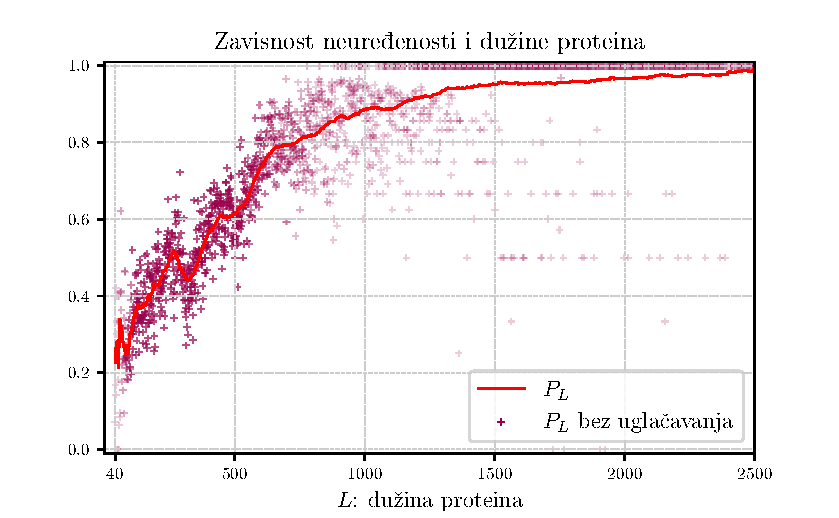
\includegraphics[]{plots/PL_F}
% \decoRule
\caption {
  Zavisnot neuređenosti i dužine CAFA3 proteina minimalne dužine 40 AK
  \footnotesize
  ($P_L$ sa prozorom uprosečavanja podrazumeva $l = 0.1L$, dok
  krstići predstavljaju diskretne vrednosti L za $l = 0$. Transparentnost krstića
  ilustruje brojnost proteina dužine $L$. Ako je krstić transparentan
  znači da sadrži manje od 100 proteina.)
}
\label{fig:PL1}
\end{figure}


Pored gore prikazanog originalnog metoda predložićemo još jedan pristup
procenjivanju veličine $P_L$.
% \keyword{Slučajno generisani} \en{random generated} proteini za procenu $P_L$.
Razmotrićemo dva modela zasnovana na slučajno generisanim proteinima. Prvi,
naivni model \keyword{uniformne verovatnoće} podrazumeva da se svaka
aminokiselina javlja sa istom verovatnoćom, odnosno $p=1/20$. U statistici je ovaj
model još poznat kao model jednakih verovatnoća \en{equiprobable model
(EPM)}.  Drugi model koji ćemo zvati slučajni ili \textit{random} model RM)  predstavlja
slučajnu promenljivu čija verovatnoća zavisi od učestalosti aminokiselina iz
CAFA3 skupa i prikazana je na Slici \ref{fig:AK_ucestalost}.
% Koristeći ova dva modela za svaki protein generisan je slučajan protein iste
% dužine koji se koristi za procenu $P_L$.
Na osnovu predstavljenih modela definisana su dva nova skupa sekvenci (EPMS i
RMS) iste kardinalnosti kao polazni CAFA3 skup, u kojima su sekvence bile istih
dužina kao u polaznom skupu. U EPMS, sekvence su generisane na osnovu uniformne
raspodele nukleotida, dok su u RMS sekvence definisane na osnovu učestalosti
aminokiselina iz CAFA3 skupa.


\begin{figure}[th]
\centering
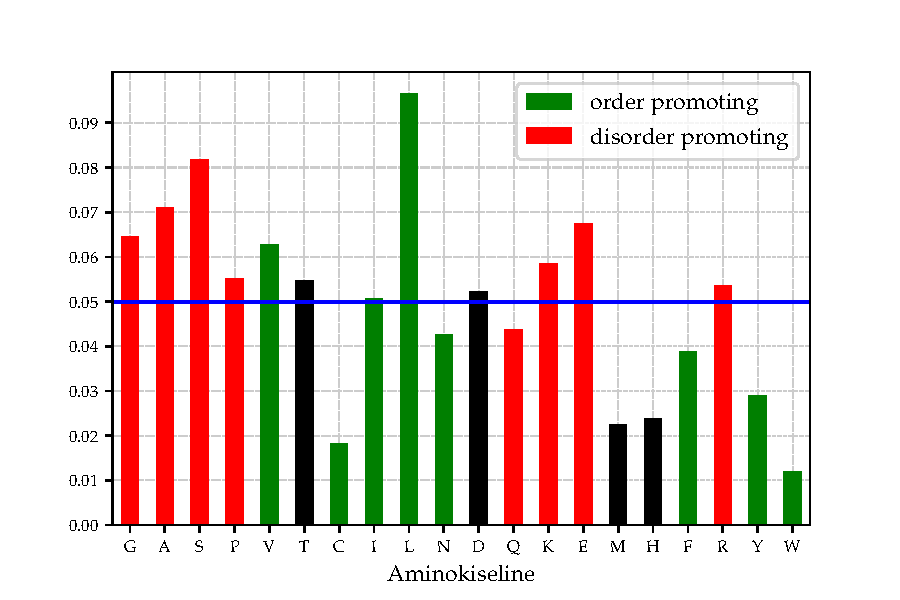
\includegraphics[]{plots/AK_ucestalost}
% \decoRule
\caption{
  Učestalost aminokiselina u CAFA3 podacima
  \\ \footnotesize
  (Učestalost prikazuje uniformni model, dok boja AK obeležava afinitet prema
  uređenosti ili neuređenosti. Aminokiseline su poređane u rastućem poretku
  od najlakše do najteže. 
}
\label{fig:AK_ucestalost}
\end{figure}

Poređenje predloženih modela sa originalnim $P_L$ prikazano je na Slici
\ref{fig:PL2}. Jasno se vidi da slučajni model predstavlja vizuelno dobru
aproksimaciju dok uniformni model znatno odstupa rastući sporije (naizgled
skoro linearno).
% Kako VSL2b prediktor prepoznaje neuređene regione na osnovu učestalosti
% aminokiselina, ovo ponašanje nije čudno jer je manja verovatnoća pojave
% aminokiselina koje promovišu neuređenost.
Zbog znatnog vizuelnog odstupanja uniformni model nije korišćen u daljoj analizi.


\begin{figure}[th]
\centering
% 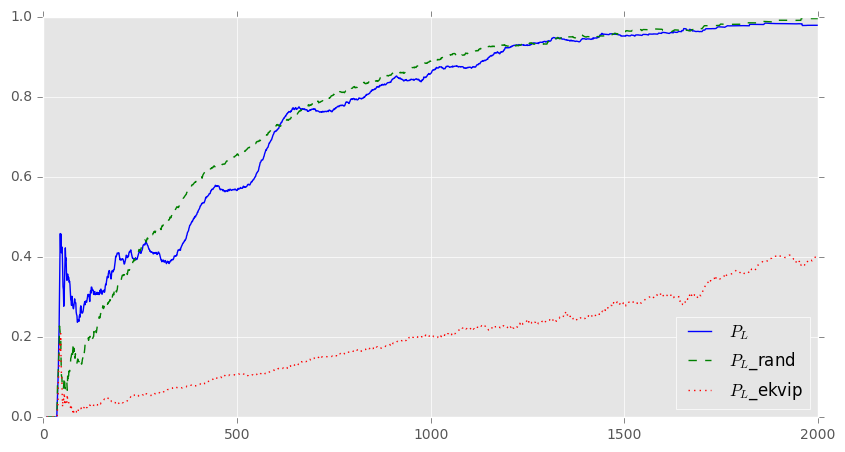
\includegraphics[scale=0.65]{Figures/PL2}
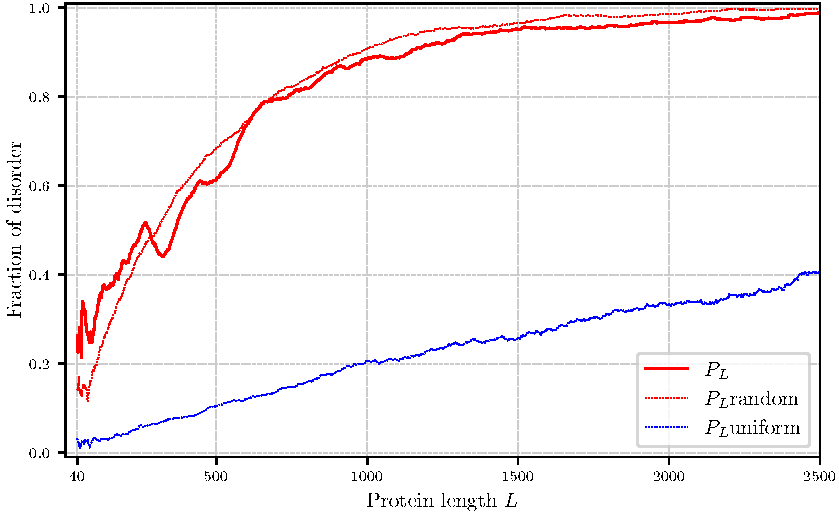
\includegraphics[]{plots/PL_F_cmp}
% \decoRule
\caption{Upoređivanje $P_L$, $P_L random$ i $P_L uniform$ modela nad CAFA3 podacima}
\label{fig:PL2}
\end{figure}


Jedno od objašnjenja zašto je uniformni model naivan i toliko odstupa od
prvobitnog metoda proizilazi iz činjenice da aminokiseline imaju inherentno
različitu učestalost u živom svetu. Naime, aminokiseline ne mogu  imati istu
verovatnoću pojavljivanja jer se  broj njihovih kodona razlikuje. Neke
aminokiseline su kodirane sa samo jednim, a druge i sa 6 kodona. Očekivano je
da veći broj kodona povećava učestalost aminokiseline i ta korelacija uz
izuzetke arginina predstavljena je Slikom \ref{fig:aminoacid}
\parencite{AKfrekvencija}.

\begin{figure}[th]
\centering
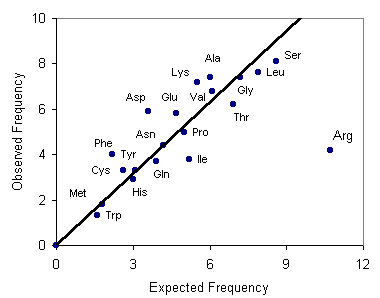
\includegraphics[scale=0.7]{aminoacid}
% \decoRule
\caption{Očekivana i izmerena učestalost aminokiselina kod kičmenjaka (preuzeto sa \cite{AA_freq_link}).  \footnotesize
  Izmerena učestalost dobijena je analizom 53 kompletno sekvencionirana proteina iz kičmenjaka \cite{King1969}.
  Očekivana učestalost kodona izračunata je kao proizvod učestalosti nukleinskih baza koje ga čine.
  Očekivana učestalost aminokiseline je zbir očekivanih učestalosti njenih kodona.
}
\label{fig:aminoacid}
\end{figure}




\clearpage
\label{ocenjivanje}
\subsection{Ocenjivanje zavisnosti funkcije od neuređenosti}

Neka je $S_j$ skup proteina koji imaju pridruženu funkciju $j$. Tada se procenat
neuređenih proteina u oznaci $F_j$ može izračunati kao:
$$F_j = \dfrac{\sum_{s_i \in S_j} d(s_i)} {|S_j|} $$



Nulta hipoteza za $F_j$ je tvrdnja da $F_j$ zavisi samo od dužine sekvence tj. $P_L$. \\
Neka je $X_L$ Bernulijeva slučajna promenljiva oblika $X_L : \begin{pmatrix} 0 & 1\\ P_L & 1-P_L \end{pmatrix}$. \\
Tada nultu hipotezu modeliramo raspodelom $Y_j$, koja za razliku od $F_j$ koristi
slučajnu promenljivu $X_L$ umesto  $d(s_i)$, odnosno:


% Nultu hiptezu koja predviđa da je rezultat $F_j$ posledica samo slučajnosti, to
% jest zavisi samo od $P_L$ opisana je preko slučajne veličine $Y_j$ gde je $X_L$
% Bernulijeva slučajna veličina sa verovatnoćom $P(X_L = 0) = P_L$ odnosno $P(X_L
% = 1) = 1-P_L$

$$ Y_j = \dfrac {\sum_{s_i \in S_j} {X_{|s_j|}}}{|S_j|}$$

Ako $F_j$ izlazi iz intervala poverenja raspodele $Y_j$ onda funkcija $j$
sadrži značajno mnogo predviđenih (ne)uređenih proteina. Preciznije,
ako je p-vrednost \en{p-value} manja od 0.05 onda je funkcija $j$ povezana sa neuređenim
proteinima, a ako je \textit{p-value} veća od 0.95 onda je funkcija $j$ povezana sa
uređenim proteinima.  Suprotno, povezanost funkcije $j$ sa (ne)uređenošću nije
statistički značajna.  

U nastavku teksta, pod neuređenošću funkcije, ključne reči ili GO termina, biće
podrazumevano da je odgovarajuća p vrednost manja od 0.05. Analogno, pod
uređenošću funkcije, ključne reči ili GO termina, biće podrazumevano da je
odgovarajuća p vrednost veća od 0.95.
% Kada se kaže da je funkcija, ključna reč ili GO termin (ne)uređen
% podrazumevaće se da je odgvorajauća p-vrednost manja od $0.05$ ili veća
% od $0.95$.

Zbog matematičkog oblika $X_L$ teško je analitički proceniti $Y_j$ pa se se
pribegava empirijskom računanju p-vrednosti. Empirijska p-vrednost određena je
tako što je za 1000 realizacija $Y_j$ izračunato očekivanje da je realizacija
$Y_j$ veća od $F_j$.

Preciznije, vektor\footnote{zamenili smo skup $S_j$ za vektor $S_j$. Ovo je
implementacioni detalj} $S_j$ sadrži $k$ proteina $S_j=\{s_1, s_2, ...
,s_{k}\}$.  Protein $s_i$ ima dužinu $L_i$ za koju je izračunata verovatnoća
$P_{L_i}$.  Tada generatorom Bernulijevih slučajnih brojeva, za svaki protein
$p_i$ na osnovu $P_{L_i}$ generišemo realizaciju $X_L$. Rezultat je vektor od
$k$ vrednosti nula ili jedan. Učestalost jedinica u rezultujućem vektoru
predstavlja prvu realizacija $Y_j$.  Postupak se ponavlja 1000 puta i broji
se koliko puta je realizacija $Y_j$ bila veća od $F_j$. Dobijeni zbir deli se
sa 1000 i rezulatat je empirijska p-vrednost.

% \begin{verbatim}
%     p = np.array( [yj>Fj for yj in Yj_1000] ).mean()
% \end{verbatim}

Originalni autori tvrde da se za veće skupove $S_j$, raspodela
$Y_j$ ponaša kao normalna. To znači da se ocena Z-skor može dobiti kao
$Z_j=(F_j-\mu_j)/\delta_j$ gde je $\mu_j$ očekivanje, a $\delta_j$ standardna
devijacija. 
% Dodatno, p-vrednost može da se aproksimira kao $1/2(1-erf(Z_j/2))$
% \footnote{$erf()$ je gausova funkcija greške,
% $erf(x)=\dfrac{2}{\sqrt{\pi}} \int_{0}^{x}  e^{-t^2} dt$ }
% ako raspodela liči na normalnu. Ovo je nekad korisno jer sa 1000 realizacija
% $Y_j$ nema dovoljnu preciznost za p vrednost manju od $1/1000=0.001$. Međutim u
% ovom radu to nije korišćeno jer su sva sortiranja (kao i u originalnom radu)
% izvršena po Z-skor oceni.




\chapter{Implementacija} % Main chapter title

\label{Implementacija} % For referencing 


%------------------------------------------------------------------------------





\chapter{Rezultati} % Main chapter title

\label{Rezultati} % For referencing 

Računarska analiza implementirana je u jeziku Pajton \en{Python} verzija 3.6.
Kompletan projekat može se naći na \textit{github} adresi \cite{projekat}. Za
potrebe projekta napravljene su dve baze podataka: relaciona baza podataka
(\textit{PostgreSQL} v9.5) i grafovska baza podataka (\textit{Neo4j} v3.1).

Od 186 MF ključnih reči koje anotiraju bar 20 proteina, 97 je statistički
značajno od čega su 53 predviđeno uređene (p<0.05), a 44 predviđeno neuređene
(p>0.95).  Od 1781 MF termina sa preko 20 pridruženih proteina (dobijeno
grupisanjem, Potpoglavnje \ref{grupisanje}), 1315 je statistički značajno od
čega su 699 predviđeno uređeni, a 616 predviđeno neuređeni.  Tabela
\ref{tab:kw_uopsteno} prikazuje razlike u odnosu na originalne rezultate.

\begin{table}[htpb]
\begin{tabular}{|r|c|c|c|}
  \hline
                     & \small originalni rezultati  & \multicolumn{2}{c|}{ novi rezultati} \\
                     & Xie2007 kw & MF kw  & MF termini                  \\
  \hline
  ukupno ($br. prot\ge20$)     & 143        & 186    & 1781                        \\
  p<0.05 (uređene)   & 37         & 53     & 699                         \\
  p>0.95 (neuređene) & 51         & 44     & 616                         \\
  \hline
\end{tabular}
  \centering
  \caption{Uopšteno poređenje rezultata}
  \label{tab:kw_uopsteno}
\end{table}

Slika \ref{fig:disorder_cmp} sadrži tri tabele predviđeno neuređenih funkcija
koje sadrže: rezultate iz originalnog rada \cite{Xie2007} (levo), nove
rezultate za MF ključne reči (sredina) i rezultate za mapirane MF termine
(desno). Sve tabele su sortirane po z-skoru opadajuće (statistička značajnost
predviđene neuređenosti opada).  Leva tabela sadrži samo 20 statistički
najznačajnije neuređenih MF ključnih reči dok je srednja ograničena na z-skor
veći od dva.  Redovi leve tabele su crveni ako se odgovarajuća ključna reč ne
nalazi u srednjoj tabeli.  Redovi srednje tabele su zeleni ako se nalaze među
prvih 20 a ključna reč se ne javlja u levoj tabeli.  Desna tabela MF termina
sadrži samo one termine koji su rezultat direktnog ili izvedenog mapiranja.
Punim strelicama prikazana su direktna mapiranja, a isprekidanim izvedena.
Nedostatak veze između srednje i desne tabele sugeriše da suprotna funkcija
nije statistički značajna, a crvena boja redova u srednjoj tabeli označava da
ni direktno ni indirektno mapiranje ne postoji.  Srednja i desna tabela pored
kolona z-skor i p vrednosti sadrže i procenat neuređenih proteina
(\text{avg\_dis}) na koji se ubuduće referišemo kao \keyword{neuređenost
funkcije}. Slike \ref{fig:disorder_cmp_ab}a, \ref{fig:disorder_cmp_ab}b
pojednostavljuju sagledavanje pojedinačnih razlika među rezultatima, međutim
zbog ograničenja formata slike neke tabele su skraćene.

Slike \ref{fig:order_cmp} i \ref{fig:order_cmp_ab}  imaju ekvivalentan format
poređenja kao i Slike \ref{fig:disorder_cmp} i \ref{fig:disorder_cmp_ab}, ali
predstavljaju sortirane uređene funkcije.



\clearpage

\begin{figure}[th]
\hspace*{-2.5cm} 
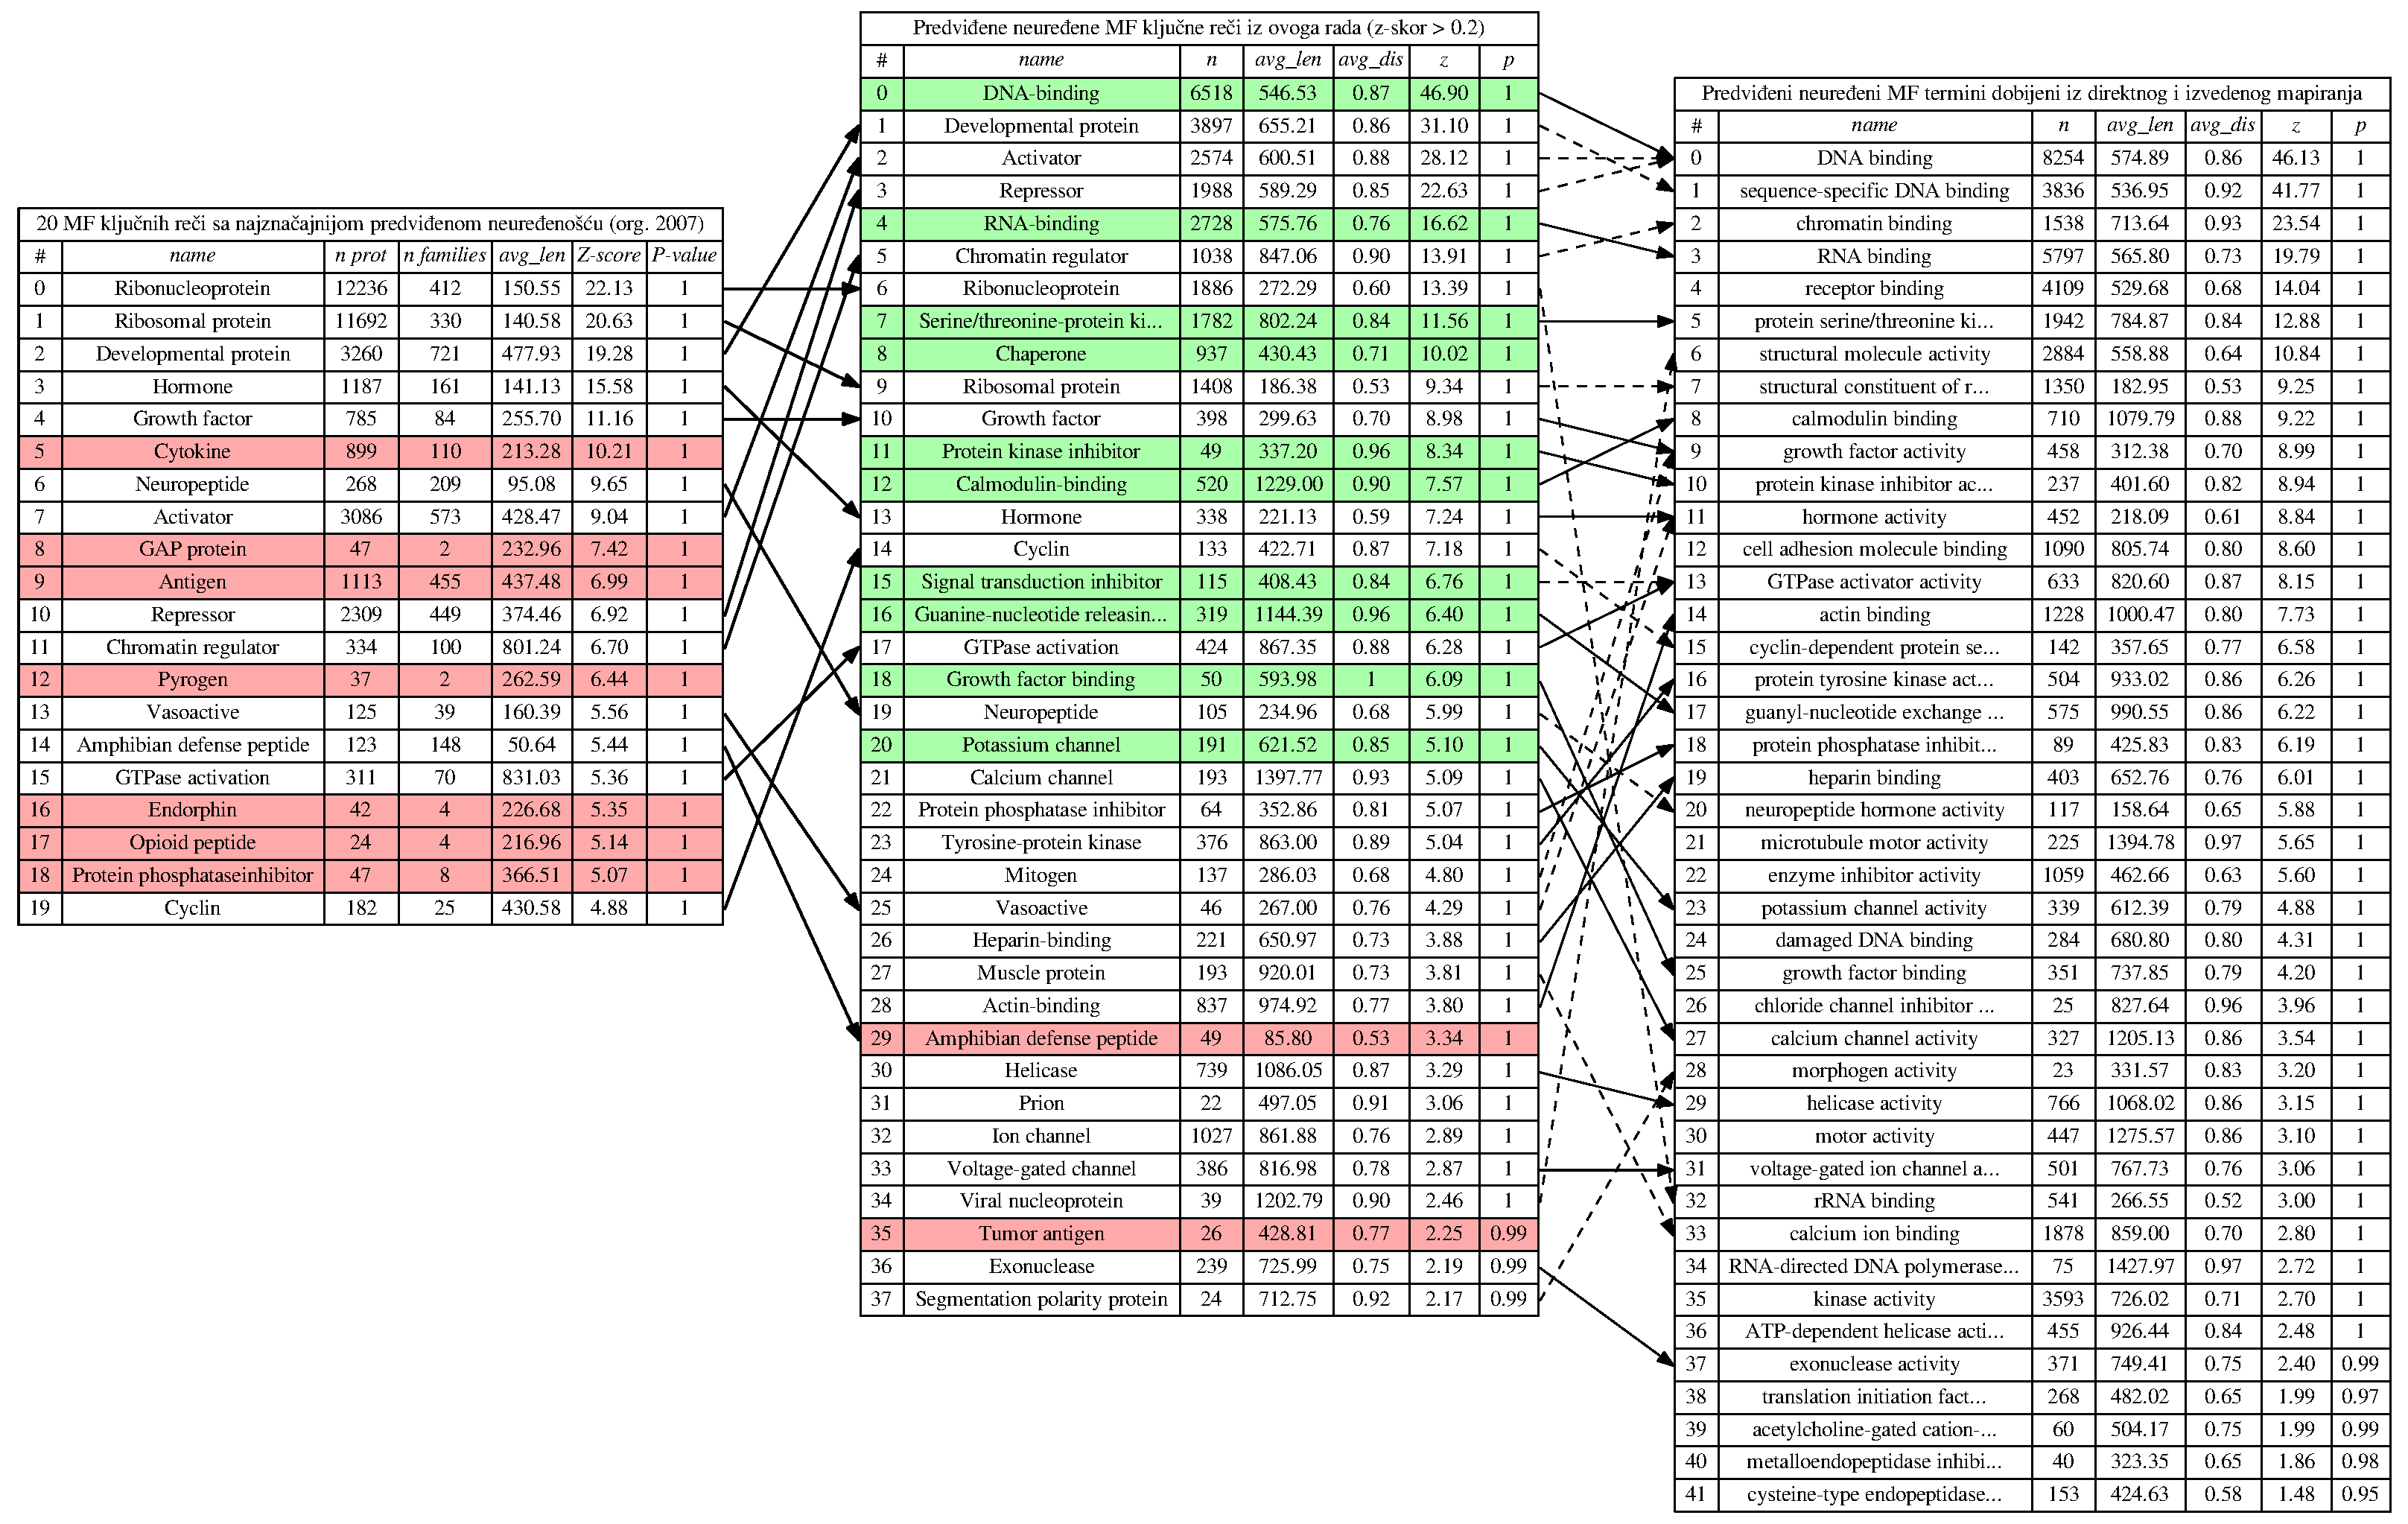
\includegraphics[angle=90, scale=0.45]{Figures/plots/disorder_cmp.pdf}
\decoRule
\caption {
  Poređenje predviđenih neuređenih funkcija
}
\label{fig:disorder_cmp}
\end{figure}

\clearpage

\begin{figure}[th]
\hspace*{-1.0cm} 
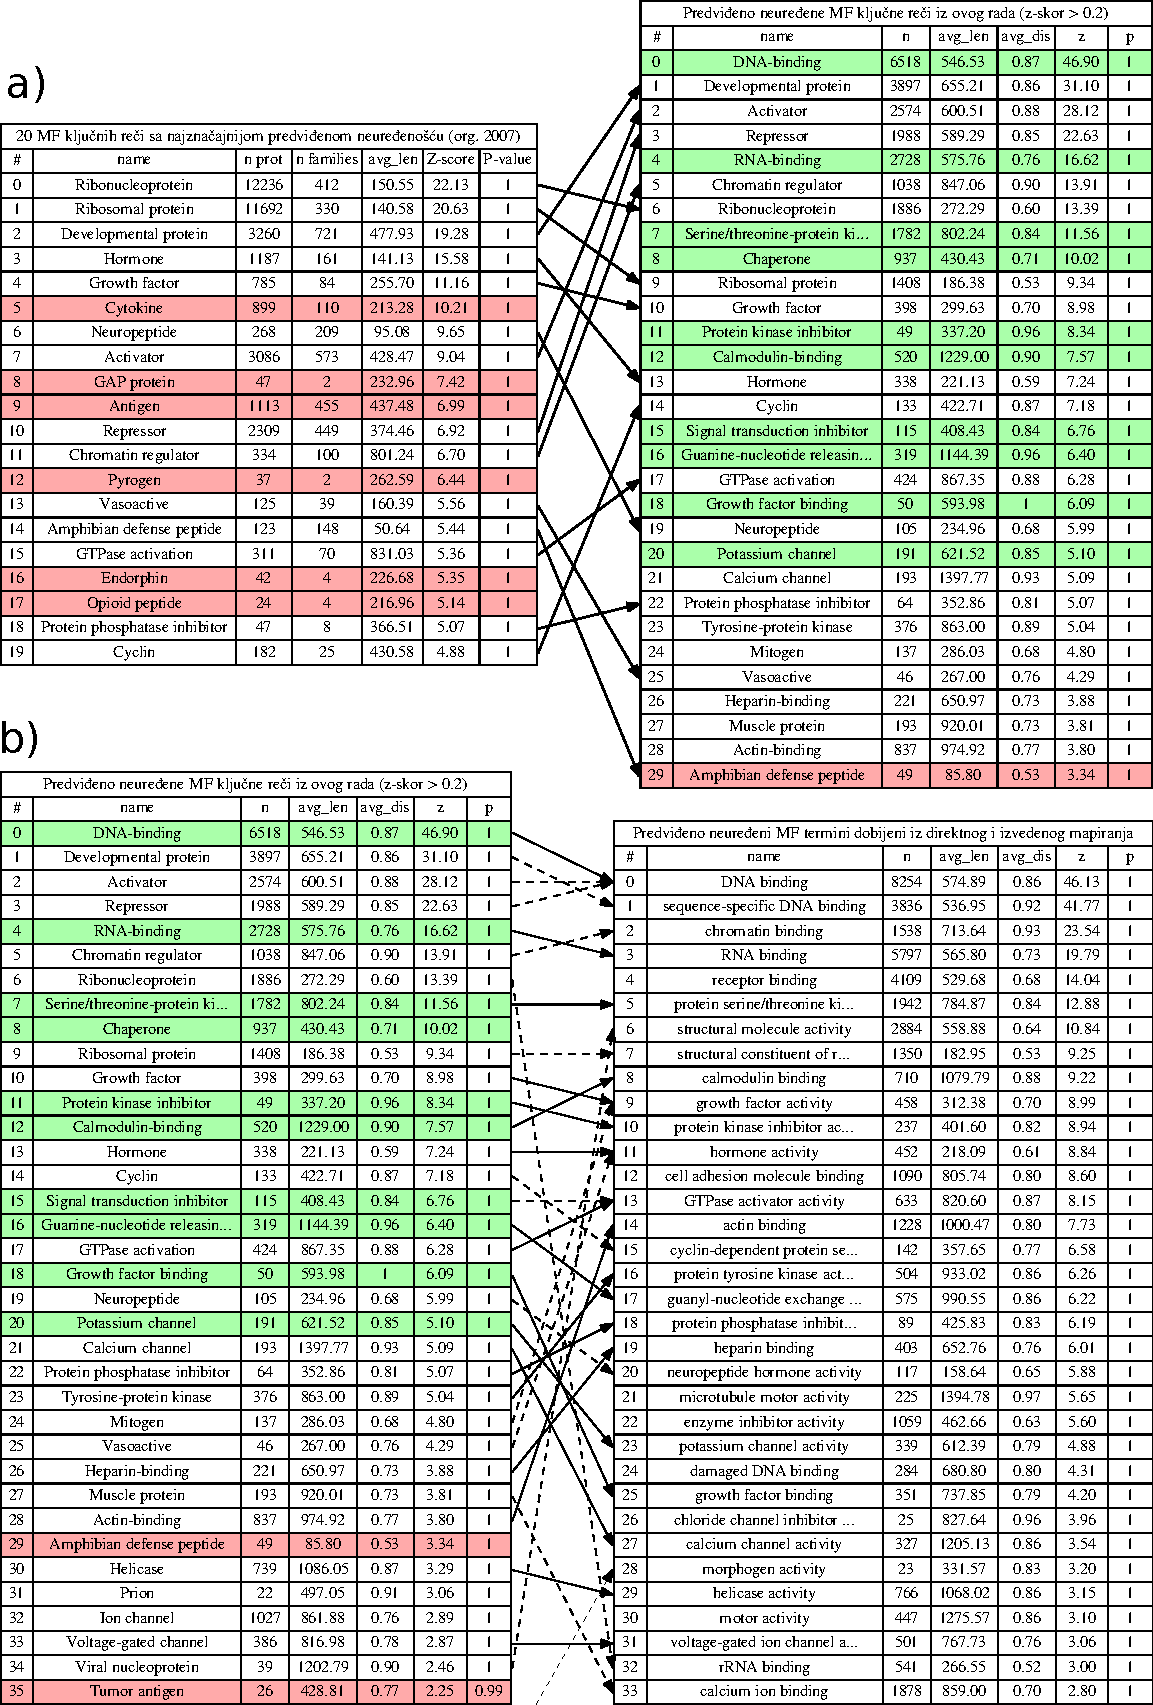
\includegraphics[ scale=0.84]{Figures/plots/disorder_cmp_ab.pdf}
\decoRule
\caption {
  Razdvojeno poređenje predviđenih neuređenih funkcija. Neke tabele su skraćene.
}
\label{fig:disorder_cmp_ab}
\end{figure}

% ------


\begin{figure}[th]
\hspace*{-2.0cm} 
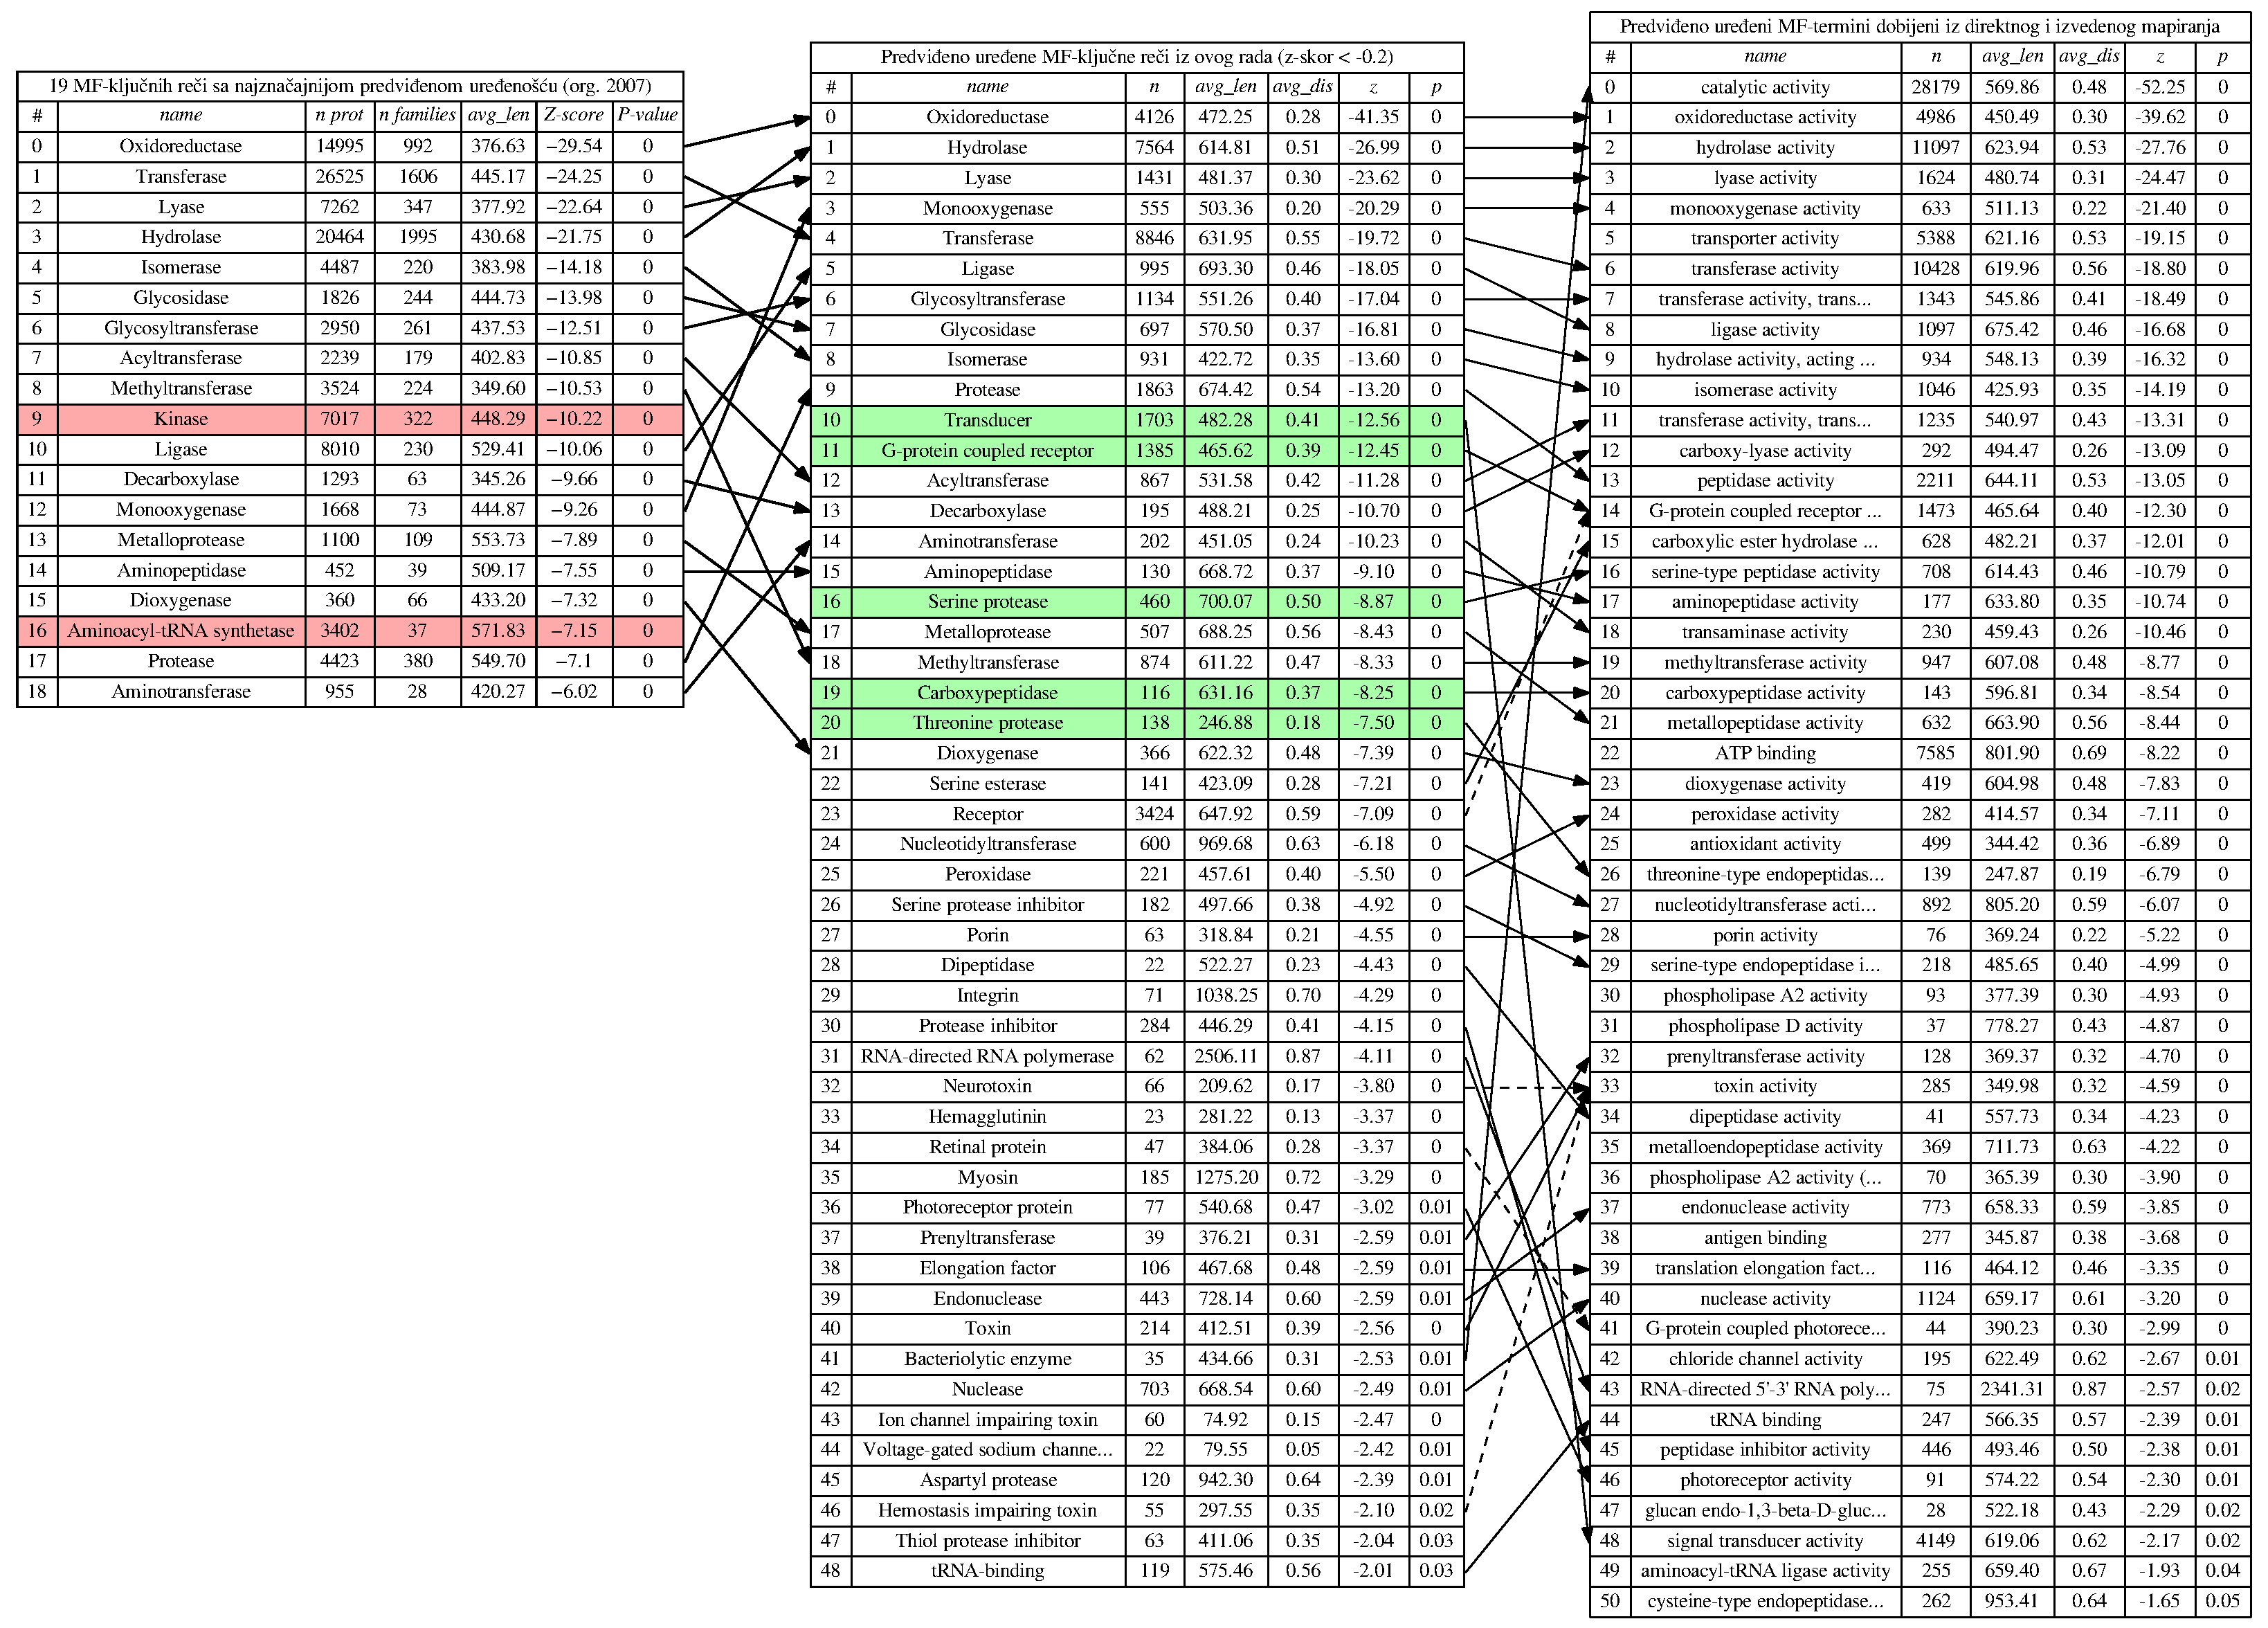
\includegraphics[angle=90, scale=0.45]{Figures/plots/order_cmp.pdf}
\decoRule
\caption {
  Poređenje predviđenih uređenih funkcija
}
\label{fig:order_cmp}
\end{figure}

\begin{figure}[th]
\hspace*{-0.5cm} 
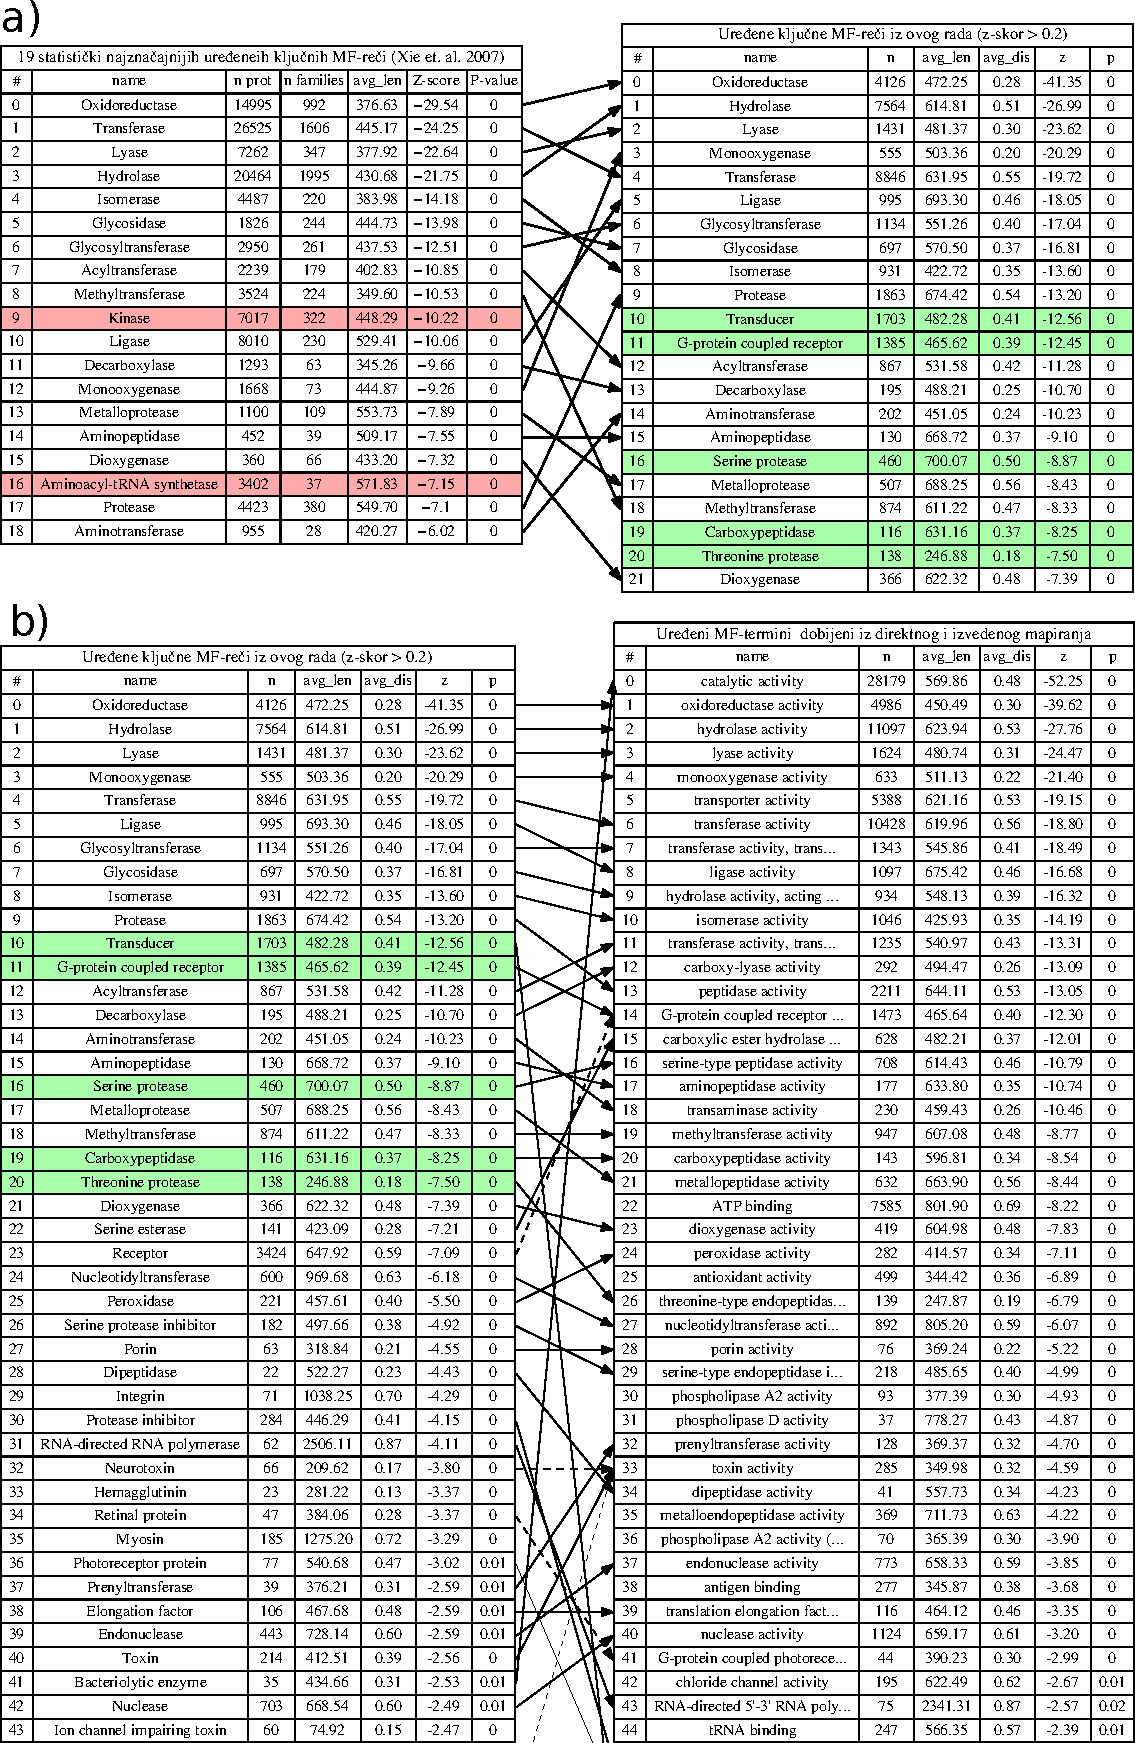
\includegraphics[scale=0.82]{Figures/plots/order_cmp_ab.pdf}
\decoRule
\caption {
  Razdvojeno poređenje predviđenih uređenih funkcija. Neke tabele su skraćene.
}
\label{fig:order_cmp_ab}
\end{figure}


\clearpage

Tabelarni pristup sa Slika \ref{fig:disorder_cmp} i \ref{fig:order_cmp}
prikazuju samo mali podskup svih statistički značajnih MF termina.  Kompletna
analiza grupisanja po MF terminima predstavljena je grafovski, slikama
\file{disorder.svg} i \file{order.svg} koje se nalaze na veb adresi
\cite{rezultati}.  Isečak rezultata \file{disorder.svg} prikazan
je Slikom \ref{fig:disorder_example}.  Pozadinska boja funkcija kodira
\keyword{neuređenost termina}, a kodirana je viridis \cite{viridis} mapiranjem
boja. Viridis mapiranje nulu predstavlja tamno ljubičastom a jedinicu svetlo
žutom pa su tamniji, plavkasti termini  uređeni dok su svetli, zelenkasti
neuređeni.  Rezultujuće \file{.svg} slike su namenjene da budu otvorene u
internet pregledaču.  Držanje kurzora miša iznad funkcija prikazaće dodatne
informacije (ime, definiciju i sinonime), dok će levi klik miša preusmeriti
korisnika na adekvatnu \textit{AmiGO}\footnote{\textit{AmiGO} je skup alat za
pretraživanje i prikazivanje GO termina } ili \uniprot veb stranicu. Desnim
klikom može da se odabere otvaranje stranice u novom tabu pregledača.

\begin{figure}[th]
\hspace*{-2.0cm} 
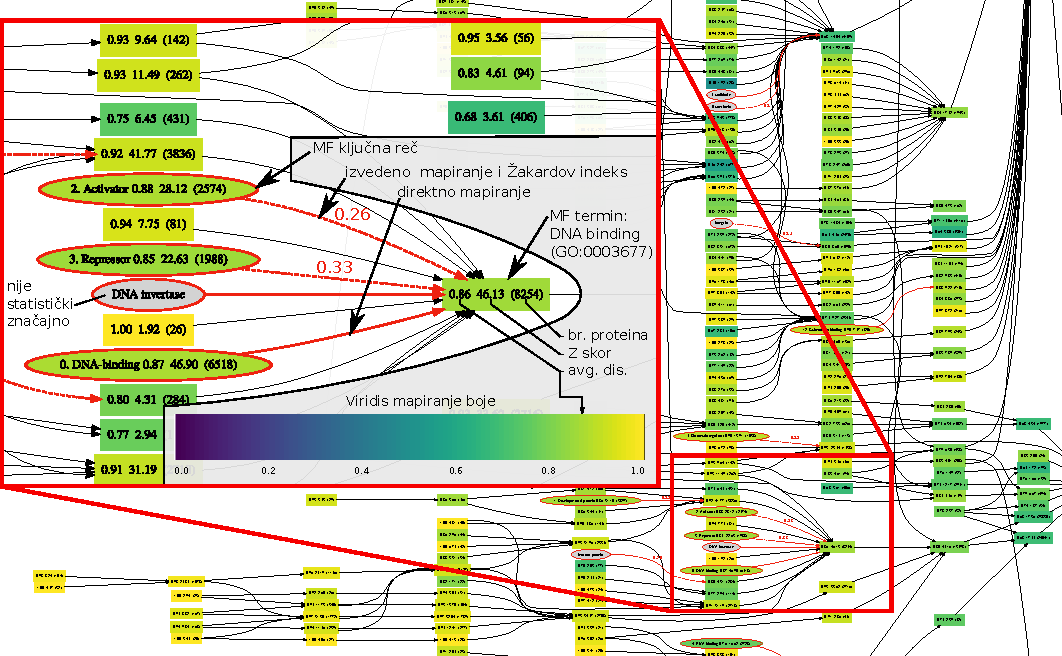
\includegraphics[angle=0, scale=1]{Figures/plots/disorder_example.pdf}
\caption {
  Isečak grafovskog prikaza rezultata (\file{disorder.png}).
}
\label{fig:disorder_example}
\end{figure}


Predloženi $P_L random$ (slučajni) model testirali smo na nivou ključnih reči
izračunavši $z_{rand}$ i  $p_{rand}$ vrednosti za sve MF ključne reči koje
anotiraju bar 20 proteina. Rezultat poređenja z skor vrednosti između $P_L$
modela ($z$-skor) i $P_L random$ modela ($z_{rand}$-skor) prikazan je na Slici
\ref{fig:PLrand}. Prikazane su samo one MF ključne reči koje su statistički
značajne u odnosu na $p$ ili $p_{rand}$ vrednosti dok su crveno obeležene one
ključne reči koje su statistički značajne po jednoj ali ne i drugoj p
vrednosti.


\begin{figure}[th]
\hspace*{-3.0cm} 
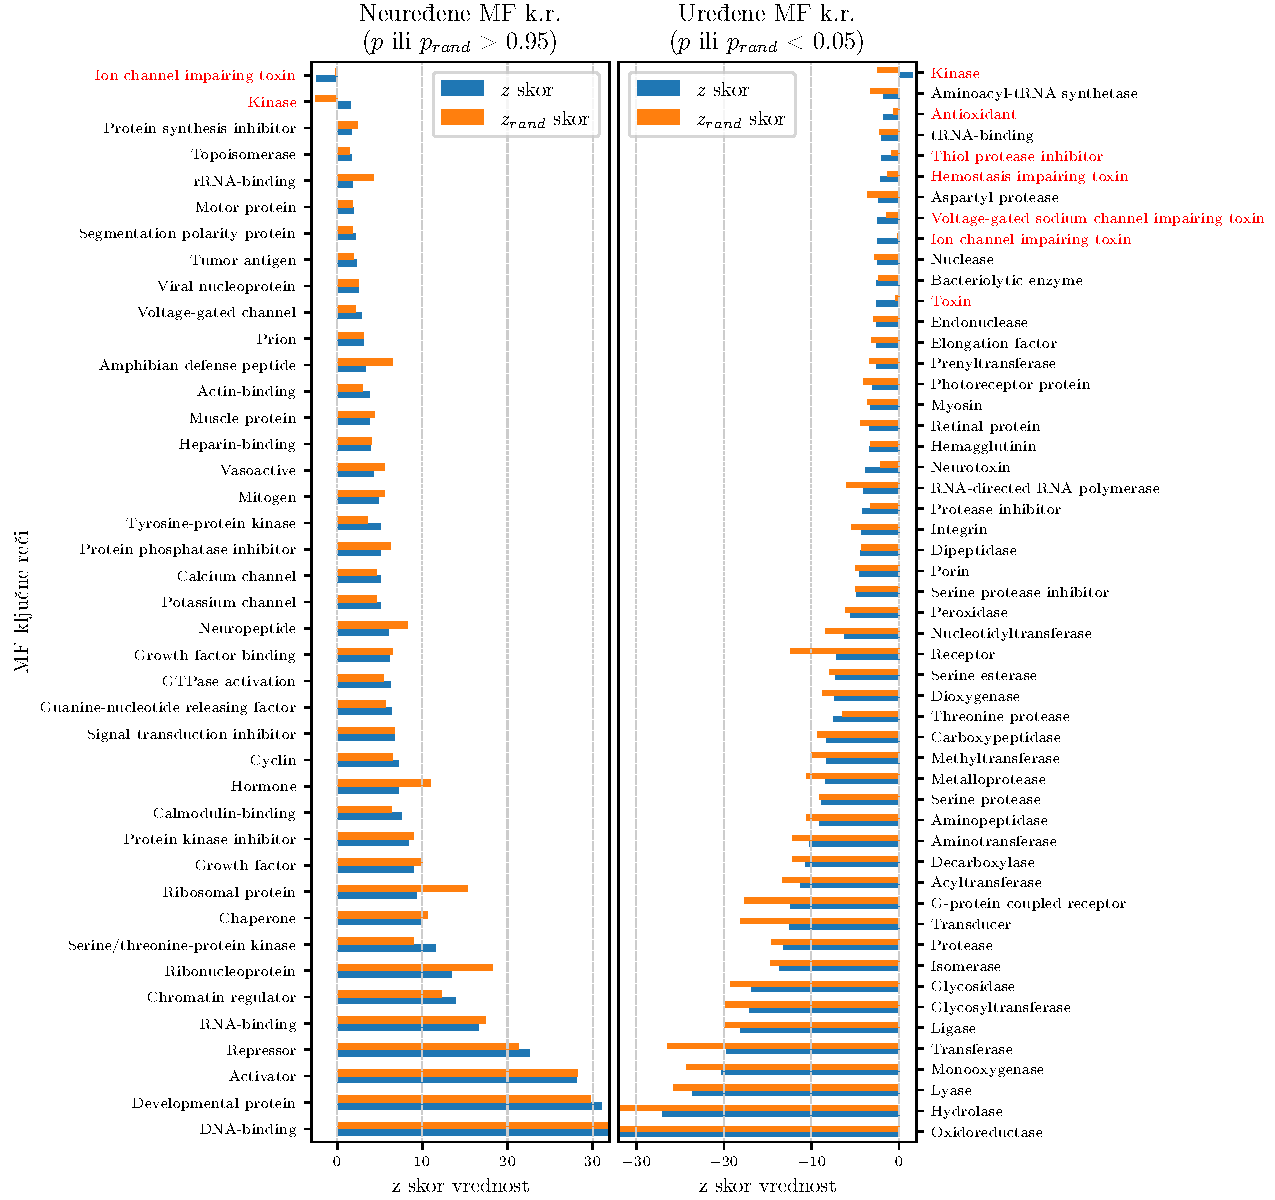
\includegraphics[angle=0, scale=1]{Figures/plots/PL_and_PL_rand.pdf}
\caption {
  Poređenje $PL$ i $PL_{random}$ modela nad statistički značajnim predviđenim (ne)uređenim MF ključnim rečima
}
\label{fig:PLrand}
\end{figure}




\chapter{Diskusija} % Main chapter title

\label{Diskusija} % For referencing 

\section{Međusobno upoređivanje MF ključnih reči}

Razmotrimo prvo Sliku \ref{fig:order_cmp_ab}a koja pokazuje da se originalni
rezultati i novi rezultati ne razlikuju bitno za predviđeno uređene MF ključne
reči. Međutim, razlike koje postoje kao i veći izuzeci (\textit{Kinase} i
\textit{Aminoacyl-tRNA synthetase} )  mogu biti posledica drugačijih podataka,
ali i modifikacije metoda originalne analize ili čak kombinacije oba faktora.
Pronalaženje egzaktnog uzorka ovih razlika zahteva dodatno istraživanje koje
prevazilazi obim ovog rada.

Sa druge strane, predviđeno \keyword{neuređene} MF ključne reči prikazane na
Slici \ref{fig:disorder_cmp_ab}a imaju znatno više razlika u odnosu na
originalne rezultate.  Šest originalnih MF ključnih reči nije identifikovano u
novim rezultatima. Ipak, \textit{Antigen} u novoj verziji ključnih reči ne
postoji dok su četiri ključne reči izbačene iz analize jer anotiraju ispod 10
CAFA3 proteina (minimum je 20).  Preostala, crvena MF ključna reč
\textit{Cytokine} ima p vrednost 0.49 što je veliko odstupanje od originalnih
rezultata. Značajnu razliku predstavljaju zeleno obeležene MF ključne reči koje
se ne javljaju u originalnim rezultatima, a nalaze se među 20 statistički
najznačajnijih novih rezultata. Među njima je preovlađujući motiv \textit{binding}, 
što se ne poklapa sa originalnim rezultatima. Za razliku od GO termina,
ključne reči ne sadrže datum dodavanja ili izmene pa ne možemo da proverimo da
li su u pitanju nove ključne reči koje nisu postojale 2006. godine.


\section{Upoređivanje MF ključnih reči i GO termina}

Rezultati prikazni Slikama \ref{fig:disorder_cmp_ab}b i
\ref{fig:order_cmp_ab}b sugerišu značajno poklapanje za statistički
najznačajnije funkcije. Kao što je očekivano, sličnost rezultata $z$-skor i
neuređenost tj. \textit{avg\_dis} pogotovo su izraženi za funkcije koje anotiraju
slične skupove proteina. Veća nepoklapanja prisutna su prvenstveno kod ključnih
reči čije je mapiranje problematično zbog razlika u nomenklaturi. Na primer,
ključna reč \textit{Bacteriolytic enzyme} nalazi se na 42. mestu dok se njen
direktno mapirani MF termin \textit{catalytic activity} nalazi na prvom mestu.

\section{Grafovski prikaz MF termina}

Grafovski prikaz na slikama \file{disorder.svg} i \file{order.svg} pruža
detaljan uvid u kompleksne hijerarhijske odnose između MF termina. Ovaj prikaz otkriva
strukture koje inače ne bi bile uočene.  Opštije MF funkcije visoke statističke
značajnosti okarakterisane su kompleksnom grafovskom strukturom potomaka. Ipak,
treba naglasiti da ovu strukturu čine isključivo statistički značajni termini
jer bi suprotno rezultat bio  teško saglediv.

\section{Statistička značajnost, neuređenost i broj proteina}

Prosek neuređenih proteina tj. \textit{avg\_dis} (neuređenost) otkriva da
funkcija ne mora da bude pretežno neuređena ili uređena da bi rezultat ($F_J$)
bio statistički značajan.  Na primer, MF termin \textit{hydrolase activity}
(Slika \ref{fig:order_cmp_ab}a) ima $z$-skor $-27.76$, međutim sadrži $53\%$
neuređenih proteina. Ipak, prosečna dužina anotiranih proteina je 624, a
verovatnoća da protein te dužine bude klasifikovan kao neuređen je 0.75.
Takođe, veličina skupa anotiranih proteina (11 097 za \textit{hydrolase
activity}) povećava statističku značajnost rezultata. Verovatno je da veliki
broj proteina smanjuje disperziju što vodi ka većim $z$-skor vrednostima.  Ovo
je posebno izraženo kod MF termina \textit{catalytic activity} na Slici
\ref{fig:order_cmp_ab}a.  Iz ovih razloga smatramo da je neophodno uzeti sve
parametre u obzir, a ne samo $z$-skor ili $p$ vrednost.

\section{$P_Lrandom$ model}

Sličnost rezultat $P_L$ i $P_L random$ modela prikazana je na Slici
\ref{fig:PLrand}. Veća odstupanja \\$z_{rand}$-skora kod ključnih reči
\textit{Ribonucleoprotein, Ribosomal protein, Hormone} i drugih ogledaju se
povećanom statističkom značajnošću. Ovo se može objasniti znatno
nižom prosečnom dužinom skupa anotiranih proteina (manje od 300 AK), dok se na
Slici \ref{fig:PL2} uočava da je $P_L random$ verovatnoća niža za proteine
kraće od 300 AK.  Obrnuto, uređene MF ključne reči globalno imaju niži
$z_{rand}$-skor (veću statističku značajnost) što se takođe može objasniti
kombinacijom globalno veće prosečne dužine proteina i većom $P_L random$
verovatnoćom (Slika \ref{fig:PL2}). 

MF ključna reč \textit{Kinase} predstavlja zanimljivo odstupanje jer $P_L
random$ model predviđa statistički značajnu uređenost iako je prosek neuređenih
proteina 0.71 i $P_L$ model predviđa neuređenost. Takođe, MF termin $Kinase
activity$ je statistički značajno neuređena ($P_L$ model).

\section{Klasifikacija neuređenog proteina}

Definicija \ref{pdis_def} neuređenosti proteina iz Potpoglavlja
\ref{naredno} nije uvek idealna.  Na primer, ako je dužina proteina 35 AK, a
neuređenost je predviđena celom dužinom, onda je jasno da nema potrebe eliminisati
protein iz analize već ga treba svrstati kao neuređeni.  Takođe, ako je protein
dug 50 AK i sadrži predviđeni neuređeni region od 35 AK, onda treba
pretpostaviti da neuređenost igra ulogu u funkciji. Ovi granični slučajevi čine
suviše mali procenat proteina u CAFA3 podksupu pa je opravdano zanemariti ih.
Međutim, procentualno \swissprot sadrži značajno više kratkih proteina što nas
navodi da istaknemo ovaj problem.

\section{Nastavak istraživanja}

Razvoj novih metaprediktora neuređenosti \cite{Meng_c2017} svakako je razlog za
nastavak istraživanja. Testiranje novih metoda analize, korišćenje drugih,
većih skupova podataka i novih metaprediktora može rezultirati interesantnim
rezultatima. Prikaz dobijenih rezultata bi trebalo da uključi razvoj
korisničkog interfejsa koji omogućuje interaktivno istraživanje, poređenje i
povezanost sa drugim resursima. Vizuelna komparacija različitih rezultata u
grafovskom obliku samo je jedan od problema koje treba rešiti.

Računarsko istraživanje veze između funkcije i tipa neuređenosti je naredni
pravac koji treba istražiti. Ipak, prediktori koji predviđaju tip neuređenosti
prema saznanjima autora još ne postoje. Iz tog razloga buduće istraživanje
treba da bude fokusirano na njihov razvoj.



\chapter{Diskusija} % Main chapter title

\label{Diskusija} % For referencing 




% % Chapter 1

\chapter{Chapter Title Here} % Main chapter title

\label{Chapter1} % For referencing the chapter elsewhere, use \ref{Chapter1} 

%----------------------------------------------------------------------------------------

% Define some commands to keep the formatting separated from the content 
% \newcommand{\keyword}[1]{\textbf{#1}}
% \newcommand{\tabhead}[1]{\textbf{#1}}
% \newcommand{\code}[1]{\texttt{#1}}
% \newcommand{\file}[1]{\texttt{\bfseries#1}}
% \newcommand{\option}[1]{\texttt{\itshape#1}}

%----------------------------------------------------------------------------------------

\section{Welcome and Thank You}
Welcome to this \LaTeX{} Thesis Template, a beautiful and easy to use template for writing a thesis using the \LaTeX{} typesetting system.

If you are writing a thesis (or will be in the future) and its subject is technical or mathematical (though it doesn't have to be), then creating it in \LaTeX{} is highly recommended as a way to make sure you can just get down to the essential writing without having to worry over formatting or wasting time arguing with your word processor.

\LaTeX{} is easily able to professionally typeset documents that run to hundreds or thousands of pages long. With simple mark-up commands, it automatically sets out the table of contents, margins, page headers and footers and keeps the formatting consistent and beautiful. One of its main strengths is the way it can easily typeset mathematics, even \emph{heavy} mathematics. Even if those equations are the most horribly twisted and most difficult mathematical problems that can only be solved on a super-computer, you can at least count on \LaTeX{} to make them look stunning.

%----------------------------------------------------------------------------------------

\section{Learning \LaTeX{}}

\LaTeX{} is not a \textsc{wysiwyg} (What You See is What You Get) program, unlike word processors such as Microsoft Word or Apple's Pages. Instead, a document written for \LaTeX{} is actually a simple, plain text file that contains \emph{no formatting}. You tell \LaTeX{} how you want the formatting in the finished document by writing in simple commands amongst the text, for example, if I want to use \emph{italic text for emphasis}, I write the \verb|\emph{text}| command and put the text I want in italics in between the curly braces. This means that \LaTeX{} is a \enquote{mark-up} language, very much like HTML.

\subsection{A (not so short) Introduction to \LaTeX{}}

If you are new to \LaTeX{}, there is a very good eBook -- freely available online as a PDF file -- called, \enquote{The Not So Short Introduction to \LaTeX{}}. The book's title is typically shortened to just \emph{lshort}. You can download the latest version (as it is occasionally updated) from here:
\url{http://www.ctan.org/tex-archive/info/lshort/english/lshort.pdf}

It is also available in several other languages. Find yours from the list on this page: \url{http://www.ctan.org/tex-archive/info/lshort/}

It is recommended to take a little time out to learn how to use \LaTeX{} by creating several, small `test' documents, or having a close look at several templates on:\\ 
\url{http://www.LaTeXTemplates.com}\\ 
Making the effort now means you're not stuck learning the system when what you \emph{really} need to be doing is writing your thesis.

\subsection{A Short Math Guide for \LaTeX{}}

If you are writing a technical or mathematical thesis, then you may want to read the document by the AMS (American Mathematical Society) called, \enquote{A Short Math Guide for \LaTeX{}}. It can be found online here:
\url{http://www.ams.org/tex/amslatex.html}
under the \enquote{Additional Documentation} section towards the bottom of the page.

\subsection{Common \LaTeX{} Math Symbols}
There are a multitude of mathematical symbols available for \LaTeX{} and it would take a great effort to learn the commands for them all. The most common ones you are likely to use are shown on this page:
\url{http://www.sunilpatel.co.uk/latex-type/latex-math-symbols/}

You can use this page as a reference or crib sheet, the symbols are rendered as large, high quality images so you can quickly find the \LaTeX{} command for the symbol you need.

\subsection{\LaTeX{} on a Mac}
 
The \LaTeX{} distribution is available for many systems including Windows, Linux and Mac OS X. The package for OS X is called MacTeX and it contains all the applications you need -- bundled together and pre-customized -- for a fully working \LaTeX{} environment and work flow.
 
MacTeX includes a custom dedicated \LaTeX{} editor called TeXShop for writing your `\file{.tex}' files and BibDesk: a program to manage your references and create your bibliography section just as easily as managing songs and creating playlists in iTunes.

%----------------------------------------------------------------------------------------

\section{Getting Started with this Template}

If you are familiar with \LaTeX{}, then you should explore the directory structure of the template and then proceed to place your own information into the \emph{THESIS INFORMATION} block of the \file{main.tex} file. You can then modify the rest of this file to your unique specifications based on your degree/university. Section \ref{FillingFile} on page \pageref{FillingFile} will help you do this. Make sure you also read section \ref{ThesisConventions} about thesis conventions to get the most out of this template.

If you are new to \LaTeX{} it is recommended that you carry on reading through the rest of the information in this document.

Before you begin using this template you should ensure that its style complies with the thesis style guidelines imposed by your institution. In most cases this template style and layout will be suitable. If it is not, it may only require a small change to bring the template in line with your institution's recommendations. These modifications will need to be done on the \file{MastersDoctoralThesis.cls} file.

\subsection{About this Template}

This \LaTeX{} Thesis Template is originally based and created around a \LaTeX{} style file created by Steve R.\ Gunn from the University of Southampton (UK), department of Electronics and Computer Science. You can find his original thesis style file at his site, here:
\url{http://www.ecs.soton.ac.uk/~srg/softwaretools/document/templates/}

Steve's \file{ecsthesis.cls} was then taken by Sunil Patel who modified it by creating a skeleton framework and folder structure to place the thesis files in. The resulting template can be found on Sunil's site here:
\url{http://www.sunilpatel.co.uk/thesis-template}

Sunil's template was made available through \url{http://www.LaTeXTemplates.com} where it was modified many times based on user requests and questions. Version 2.0 and onwards of this template represents a major modification to Sunil's template and is, in fact, hardly recognisable. The work to make version 2.0 possible was carried out by \href{mailto:vel@latextemplates.com}{Vel} and Johannes Böttcher.

%----------------------------------------------------------------------------------------

\section{What this Template Includes}

\subsection{Folders}

This template comes as a single zip file that expands out to several files and folders. The folder names are mostly self-explanatory:

\keyword{Appendices} -- this is the folder where you put the appendices. Each appendix should go into its own separate \file{.tex} file. An example and template are included in the directory.

\keyword{Chapters} -- this is the folder where you put the thesis chapters. A thesis usually has about six chapters, though there is no hard rule on this. Each chapter should go in its own separate \file{.tex} file and they can be split as:
\begin{itemize}
\item Chapter 1: Introduction to the thesis topic
\item Chapter 2: Background information and theory
\item Chapter 3: (Laboratory) experimental setup
\item Chapter 4: Details of experiment 1
\item Chapter 5: Details of experiment 2
\item Chapter 6: Discussion of the experimental results
\item Chapter 7: Conclusion and future directions
\end{itemize}
This chapter layout is specialised for the experimental sciences, your discipline may be different.

\keyword{Figures} -- this folder contains all figures for the thesis. These are the final images that will go into the thesis document.

\subsection{Files}

Included are also several files, most of them are plain text and you can see their contents in a text editor. After initial compilation, you will see that more auxiliary files are created by \LaTeX{} or BibTeX and which you don't need to delete or worry about:

\keyword{example.bib} -- this is an important file that contains all the bibliographic information and references that you will be citing in the thesis for use with BibTeX. You can write it manually, but there are reference manager programs available that will create and manage it for you. Bibliographies in \LaTeX{} are a large subject and you may need to read about BibTeX before starting with this. Many modern reference managers will allow you to export your references in BibTeX format which greatly eases the amount of work you have to do.

\keyword{MastersDoctoralThesis.cls} -- this is an important file. It is the class file that tells \LaTeX{} how to format the thesis. 

\keyword{main.pdf} -- this is your beautifully typeset thesis (in the PDF file format) created by \LaTeX{}. It is supplied in the PDF with the template and after you compile the template you should get an identical version.

\keyword{main.tex} -- this is an important file. This is the file that you tell \LaTeX{} to compile to produce your thesis as a PDF file. It contains the framework and constructs that tell \LaTeX{} how to layout the thesis. It is heavily commented so you can read exactly what each line of code does and why it is there. After you put your own information into the \emph{THESIS INFORMATION} block -- you have now started your thesis!

Files that are \emph{not} included, but are created by \LaTeX{} as auxiliary files include:

\keyword{main.aux} -- this is an auxiliary file generated by \LaTeX{}, if it is deleted \LaTeX{} simply regenerates it when you run the main \file{.tex} file.

\keyword{main.bbl} -- this is an auxiliary file generated by BibTeX, if it is deleted, BibTeX simply regenerates it when you run the \file{main.aux} file. Whereas the \file{.bib} file contains all the references you have, this \file{.bbl} file contains the references you have actually cited in the thesis and is used to build the bibliography section of the thesis.

\keyword{main.blg} -- this is an auxiliary file generated by BibTeX, if it is deleted BibTeX simply regenerates it when you run the main \file{.aux} file.

\keyword{main.lof} -- this is an auxiliary file generated by \LaTeX{}, if it is deleted \LaTeX{} simply regenerates it when you run the main \file{.tex} file. It tells \LaTeX{} how to build the \emph{List of Figures} section.

\keyword{main.log} -- this is an auxiliary file generated by \LaTeX{}, if it is deleted \LaTeX{} simply regenerates it when you run the main \file{.tex} file. It contains messages from \LaTeX{}, if you receive errors and warnings from \LaTeX{}, they will be in this \file{.log} file.

\keyword{main.lot} -- this is an auxiliary file generated by \LaTeX{}, if it is deleted \LaTeX{} simply regenerates it when you run the main \file{.tex} file. It tells \LaTeX{} how to build the \emph{List of Tables} section.

\keyword{main.out} -- this is an auxiliary file generated by \LaTeX{}, if it is deleted \LaTeX{} simply regenerates it when you run the main \file{.tex} file.

So from this long list, only the files with the \file{.bib}, \file{.cls} and \file{.tex} extensions are the most important ones. The other auxiliary files can be ignored or deleted as \LaTeX{} and BibTeX will regenerate them.

%----------------------------------------------------------------------------------------

\section{Filling in Your Information in the \file{main.tex} File}\label{FillingFile}

You will need to personalise the thesis template and make it your own by filling in your own information. This is done by editing the \file{main.tex} file in a text editor or your favourite LaTeX environment.

Open the file and scroll down to the third large block titled \emph{THESIS INFORMATION} where you can see the entries for \emph{University Name}, \emph{Department Name}, etc \ldots

Fill out the information about yourself, your group and institution. You can also insert web links, if you do, make sure you use the full URL, including the \code{http://} for this. If you don't want these to be linked, simply remove the \verb|\href{url}{name}| and only leave the name.

When you have done this, save the file and recompile \code{main.tex}. All the information you filled in should now be in the PDF, complete with web links. You can now begin your thesis proper!

%----------------------------------------------------------------------------------------

\section{The \code{main.tex} File Explained}

The \file{main.tex} file contains the structure of the thesis. There are plenty of written comments that explain what pages, sections and formatting the \LaTeX{} code is creating. Each major document element is divided into commented blocks with titles in all capitals to make it obvious what the following bit of code is doing. Initially there seems to be a lot of \LaTeX{} code, but this is all formatting, and it has all been taken care of so you don't have to do it.

Begin by checking that your information on the title page is correct. For the thesis declaration, your institution may insist on something different than the text given. If this is the case, just replace what you see with what is required in the \emph{DECLARATION PAGE} block.

Then comes a page which contains a funny quote. You can put your own, or quote your favourite scientist, author, person, and so on. Make sure to put the name of the person who you took the quote from.

Following this is the abstract page which summarises your work in a condensed way and can almost be used as a standalone document to describe what you have done. The text you write will cause the heading to move up so don't worry about running out of space.

Next come the acknowledgements. On this page, write about all the people who you wish to thank (not forgetting parents, partners and your advisor/supervisor).

The contents pages, list of figures and tables are all taken care of for you and do not need to be manually created or edited. The next set of pages are more likely to be optional and can be deleted since they are for a more technical thesis: insert a list of abbreviations you have used in the thesis, then a list of the physical constants and numbers you refer to and finally, a list of mathematical symbols used in any formulae. Making the effort to fill these tables means the reader has a one-stop place to refer to instead of searching the internet and references to try and find out what you meant by certain abbreviations or symbols.

The list of symbols is split into the Roman and Greek alphabets. Whereas the abbreviations and symbols ought to be listed in alphabetical order (and this is \emph{not} done automatically for you) the list of physical constants should be grouped into similar themes.

The next page contains a one line dedication. Who will you dedicate your thesis to?

Finally, there is the block where the chapters are included. Uncomment the lines (delete the \code{\%} character) as you write the chapters. Each chapter should be written in its own file and put into the \emph{Chapters} folder and named \file{Chapter1}, \file{Chapter2}, etc\ldots Similarly for the appendices, uncomment the lines as you need them. Each appendix should go into its own file and placed in the \emph{Appendices} folder.

After the preamble, chapters and appendices finally comes the bibliography. The bibliography style (called \option{authoryear}) is used for the bibliography and is a fully featured style that will even include links to where the referenced paper can be found online. Do not underestimate how grateful your reader will be to find that a reference to a paper is just a click away. Of course, this relies on you putting the URL information into the BibTeX file in the first place.

%----------------------------------------------------------------------------------------

\section{Thesis Features and Conventions}\label{ThesisConventions}

To get the best out of this template, there are a few conventions that you may want to follow.

One of the most important (and most difficult) things to keep track of in such a long document as a thesis is consistency. Using certain conventions and ways of doing things (such as using a Todo list) makes the job easier. Of course, all of these are optional and you can adopt your own method.

\subsection{Printing Format}

This thesis template is designed for double sided printing (i.e. content on the front and back of pages) as most theses are printed and bound this way. Switching to one sided printing is as simple as uncommenting the \option{oneside} option of the \code{documentclass} command at the top of the \file{main.tex} file. You may then wish to adjust the margins to suit specifications from your institution.

The headers for the pages contain the page number on the outer side (so it is easy to flick through to the page you want) and the chapter name on the inner side.

The text is set to 11 point by default with single line spacing, again, you can tune the text size and spacing should you want or need to using the options at the very start of \file{main.tex}. The spacing can be changed similarly by replacing the \option{singlespacing} with \option{onehalfspacing} or \option{doublespacing}.

\subsection{Using US Letter Paper}

The paper size used in the template is A4, which is the standard size in Europe. If you are using this thesis template elsewhere and particularly in the United States, then you may have to change the A4 paper size to the US Letter size. This can be done in the margins settings section in \file{main.tex}.

Due to the differences in the paper size, the resulting margins may be different to what you like or require (as it is common for institutions to dictate certain margin sizes). If this is the case, then the margin sizes can be tweaked by modifying the values in the same block as where you set the paper size. Now your document should be set up for US Letter paper size with suitable margins.

\subsection{References}

The \code{biblatex} package is used to format the bibliography and inserts references such as this one \parencite{Reference1}. The options used in the \file{main.tex} file mean that the in-text citations of references are formatted with the author(s) listed with the date of the publication. Multiple references are separated by semicolons (e.g. \parencite{Reference2, Reference1}) and references with more than three authors only show the first author with \emph{et al.} indicating there are more authors (e.g. \parencite{Reference3}). This is done automatically for you. To see how you use references, have a look at the \file{Chapter1.tex} source file. Many reference managers allow you to simply drag the reference into the document as you type.

Scientific references should come \emph{before} the punctuation mark if there is one (such as a comma or period). The same goes for footnotes\footnote{Such as this footnote, here down at the bottom of the page.}. You can change this but the most important thing is to keep the convention consistent throughout the thesis. Footnotes themselves should be full, descriptive sentences (beginning with a capital letter and ending with a full stop). The APA6 states: \enquote{Footnote numbers should be superscripted, [...], following any punctuation mark except a dash.} The Chicago manual of style states: \enquote{A note number should be placed at the end of a sentence or clause. The number follows any punctuation mark except the dash, which it precedes. It follows a closing parenthesis.}

The bibliography is typeset with references listed in alphabetical order by the first author's last name. This is similar to the APA referencing style. To see how \LaTeX{} typesets the bibliography, have a look at the very end of this document (or just click on the reference number links in in-text citations).

\subsubsection{A Note on bibtex}

The bibtex backend used in the template by default does not correctly handle unicode character encoding (i.e. "international" characters). You may see a warning about this in the compilation log and, if your references contain unicode characters, they may not show up correctly or at all. The solution to this is to use the biber backend instead of the outdated bibtex backend. This is done by finding this in \file{main.tex}: \option{backend=bibtex} and changing it to \option{backend=biber}. You will then need to delete all auxiliary BibTeX files and navigate to the template directory in your terminal (command prompt). Once there, simply type \code{biber main} and biber will compile your bibliography. You can then compile \file{main.tex} as normal and your bibliography will be updated. An alternative is to set up your LaTeX editor to compile with biber instead of bibtex, see \href{http://tex.stackexchange.com/questions/154751/biblatex-with-biber-configuring-my-editor-to-avoid-undefined-citations/}{here} for how to do this for various editors.

\subsection{Tables}

Tables are an important way of displaying your results, below is an example table which was generated with this code:

{\small
\begin{verbatim}
\begin{table}
\caption{The effects of treatments X and Y on the four groups studied.}
\label{tab:treatments}
\centering
\begin{tabular}{l l l}
\toprule
\tabhead{Groups} & \tabhead{Treatment X} & \tabhead{Treatment Y} \\
\midrule
1 & 0.2 & 0.8\\
2 & 0.17 & 0.7\\
3 & 0.24 & 0.75\\
4 & 0.68 & 0.3\\
\bottomrule\\
\end{tabular}
\end{table}
\end{verbatim}
}

\begin{table}
\caption{The effects of treatments X and Y on the four groups studied.}
\label{tab:treatments}
\centering
\begin{tabular}{l l l}
\toprule
\tabhead{Groups} & \tabhead{Treatment X} & \tabhead{Treatment Y} \\
\midrule
1 & 0.2 & 0.8\\
2 & 0.17 & 0.7\\
3 & 0.24 & 0.75\\
4 & 0.68 & 0.3\\
\bottomrule\\
\end{tabular}
\end{table}

You can reference tables with \verb|\ref{<label>}| where the label is defined within the table environment. See \file{Chapter1.tex} for an example of the label and citation (e.g. Table~\ref{tab:treatments}).

\subsection{Figures}

There will hopefully be many figures in your thesis (that should be placed in the \emph{Figures} folder). The way to insert figures into your thesis is to use a code template like this:
\begin{verbatim}
\begin{figure}
\centering
\includegraphics{Figures/Electron}
\decoRule
\caption[An Electron]{An electron (artist's impression).}
\label{fig:Electron}
\end{figure}
\end{verbatim}
Also look in the source file. Putting this code into the source file produces the picture of the electron that you can see in the figure below.

\begin{figure}[th]
\centering
\includegraphics{Figures/Electron}
\decoRule
\caption[An Electron]{An electron (artist's impression).}
\label{fig:Electron}
\end{figure}

Sometimes figures don't always appear where you write them in the source. The placement depends on how much space there is on the page for the figure. Sometimes there is not enough room to fit a figure directly where it should go (in relation to the text) and so \LaTeX{} puts it at the top of the next page. Positioning figures is the job of \LaTeX{} and so you should only worry about making them look good!

Figures usually should have captions just in case you need to refer to them (such as in Figure~\ref{fig:Electron}). The \verb|\caption| command contains two parts, the first part, inside the square brackets is the title that will appear in the \emph{List of Figures}, and so should be short. The second part in the curly brackets should contain the longer and more descriptive caption text.

The \verb|\decoRule| command is optional and simply puts an aesthetic horizontal line below the image. If you do this for one image, do it for all of them.

\LaTeX{} is capable of using images in pdf, jpg and png format.

\subsection{Typesetting mathematics}

If your thesis is going to contain heavy mathematical content, be sure that \LaTeX{} will make it look beautiful, even though it won't be able to solve the equations for you.

The \enquote{Not So Short Introduction to \LaTeX} (available on \href{http://www.ctan.org/tex-archive/info/lshort/english/lshort.pdf}{CTAN}) should tell you everything you need to know for most cases of typesetting mathematics. If you need more information, a much more thorough mathematical guide is available from the AMS called, \enquote{A Short Math Guide to \LaTeX} and can be downloaded from:
\url{ftp://ftp.ams.org/pub/tex/doc/amsmath/short-math-guide.pdf}

There are many different \LaTeX{} symbols to remember, luckily you can find the most common symbols in \href{http://ctan.org/pkg/comprehensive}{The Comprehensive \LaTeX~Symbol List}.

You can write an equation, which is automatically given an equation number by \LaTeX{} like this:
\begin{verbatim}
\begin{equation}
E = mc^{2}
\label{eqn:Einstein}
\end{equation}
\end{verbatim}

This will produce Einstein's famous energy-matter equivalence equation:
\begin{equation}
E = mc^{2}
\label{eqn:Einstein}
\end{equation}

All equations you write (which are not in the middle of paragraph text) are automatically given equation numbers by \LaTeX{}. If you don't want a particular equation numbered, use the unnumbered form:
\begin{verbatim}
\[ a^{2}=4 \]
\end{verbatim}

%----------------------------------------------------------------------------------------

\section{Sectioning and Subsectioning}

You should break your thesis up into nice, bite-sized sections and subsections. \LaTeX{} automatically builds a table of Contents by looking at all the \verb|\chapter{}|, \verb|\section{}|  and \verb|\subsection{}| commands you write in the source.

The Table of Contents should only list the sections to three (3) levels. A \verb|chapter{}| is level zero (0). A \verb|\section{}| is level one (1) and so a \verb|\subsection{}| is level two (2). In your thesis it is likely that you will even use a \verb|subsubsection{}|, which is level three (3). The depth to which the Table of Contents is formatted is set within \file{MastersDoctoralThesis.cls}. If you need this changed, you can do it in \file{main.tex}.

%----------------------------------------------------------------------------------------

\section{In Closing}

You have reached the end of this mini-guide. You can now rename or overwrite this pdf file and begin writing your own \file{Chapter1.tex} and the rest of your thesis. The easy work of setting up the structure and framework has been taken care of for you. It's now your job to fill it out!

Good luck and have lots of fun!

\begin{flushright}
Guide written by ---\\
Sunil Patel: \href{http://www.sunilpatel.co.uk}{www.sunilpatel.co.uk}\\
Vel: \href{http://www.LaTeXTemplates.com}{LaTeXTemplates.com}
\end{flushright}

% \include{Chapters/Chapter2} 
%\include{Chapters/Chapter3}
%\include{Chapters/Chapter4} 
%\include{Chapters/Chapter5} 

%----------------------------------------------------------------------------------------
%	THESIS CONTENT - APPENDICES
%----------------------------------------------------------------------------------------

\appendix % Cue to tell LaTeX that the following "chapters" are Appendices

% Include the appendices of the thesis as separate files from the Appendices folder
% Uncomment the lines as you write the Appendices

% % Appendix A

\chapter{Frequently Asked Questions} % Main appendix title

\label{AppendixA} % For referencing this appendix elsewhere, use \ref{AppendixA}

\section{How do I change the colors of links?}

The color of links can be changed to your liking using:

{\small\verb!\hypersetup{urlcolor=red}!}, or

{\small\verb!\hypersetup{citecolor=green}!}, or

{\small\verb!\hypersetup{allcolor=blue}!}.

\noindent If you want to completely hide the links, you can use:

{\small\verb!\hypersetup{allcolors=.}!}, or even better: 

{\small\verb!\hypersetup{hidelinks}!}.

\noindent If you want to have obvious links in the PDF but not the printed text, use:

{\small\verb!\hypersetup{colorlinks=false}!}.

%\include{Appendices/AppendixB}
%\include{Appendices/AppendixC}

%----------------------------------------------------------------------------------------
%	BIBLIOGRAPHY
%----------------------------------------------------------------------------------------

\renewcommand{\bibname}{Bibliografija}

\printbibliography[heading=bibintoc]

%----------------------------------------------------------------------------------------

\end{document}  
